\documentclass[a4paper,11pt]{book}
\usepackage[top=3.5cm, bottom=3.5cm, left=3.5cm, right=3.5cm]{geometry}\usepackage[T1]{fontenc}
\usepackage[utf8]{inputenc}
\usepackage[english]{babel}
\usepackage{lmodern}
\usepackage{amsmath}
\usepackage{amsfonts}
\usepackage{amssymb}
\usepackage{amsthm}
\usepackage{array}
\usepackage{graphicx}
\usepackage{color}
\usepackage{xcolor}
\usepackage{url}
\usepackage{theorem}
\usepackage{textcomp}
\usepackage{listings}
\usepackage{hyperref}
\usepackage{parskip}
\usepackage{tikz}
\usepackage{float}
\usepackage{fancybox}
\usepackage{fancyhdr}
\usepackage{cancel}
\usepackage{subcaption}
\usepackage{caption}
\usepackage{adjustbox}
\usepackage{csquotes}
\usepackage{nth}
\pagestyle{fancy}
\fancyhf{}
\fancyhead[LE,RO]{\thepage}
\fancyhead[RE]{\leftmark}
\fancyhead[LO]{\rightmark}

\renewcommand{\chaptermark}[1]{\markboth{Chapter \thechapter: #1}{}}

\graphicspath{{Sketches/}}


\newcommand{\doctitle}{Fluid Mechanics}
\newcommand{\docauthor}{Course of Tobias Schneider\\Trancription by Tim Tschanz}

\title{\doctitle}
\author{\docauthor}
\date{\today}

\hypersetup{
    pdftitle={\doctitle},
    pdfauthor={\docauthor},
}

\setlength{\headheight}{13.6pt}


\begin{document}
\begin{titlepage}
	\centering
	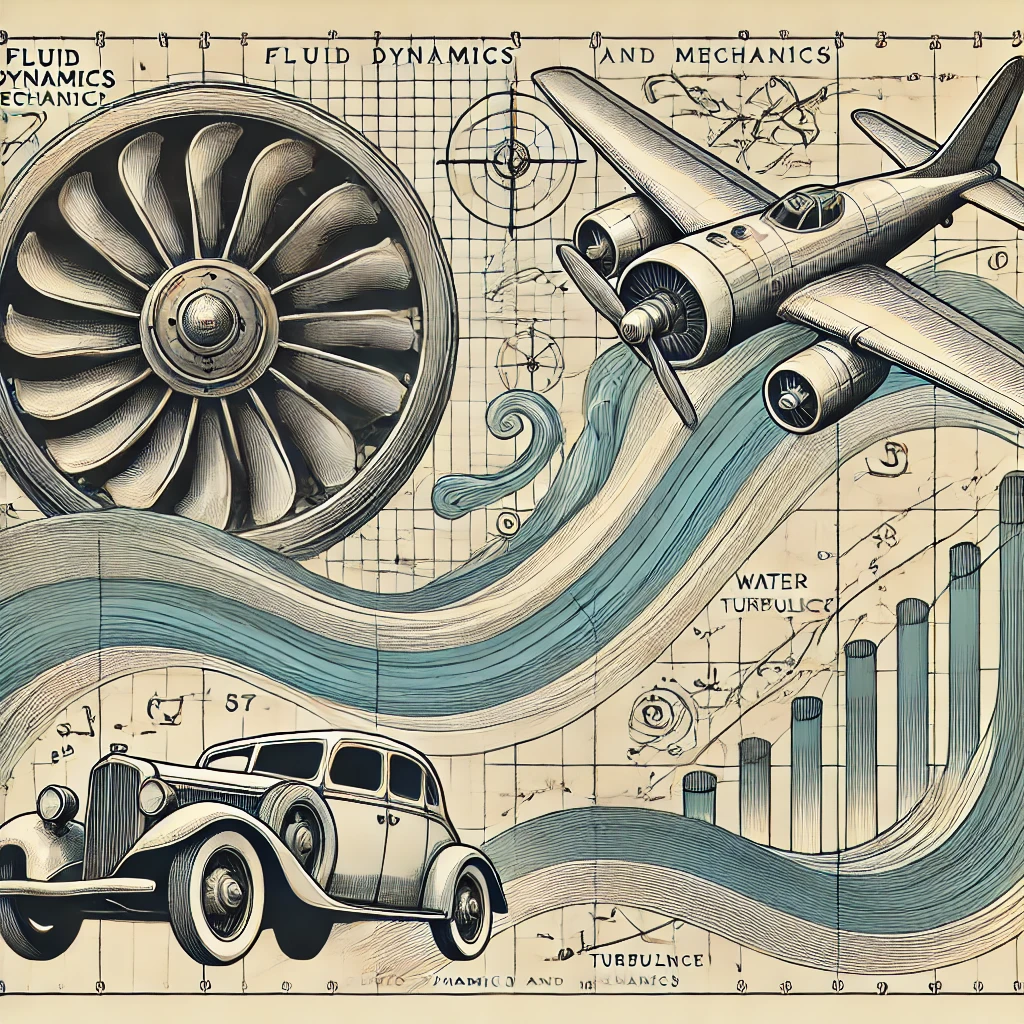
\includegraphics[width=\textwidth]{Cover_Image.png}
	{\huge\bfseries \doctitle\par}
	{
		\vspace{1cm}
		{\large \docauthor\par}
		\vspace{1cm}
	}
	{\large \today\par}
\end{titlepage}

\tableofcontents

\chapter{Introduction}

This chapter is based on Munson Chapter 1.
\section{Definitions}
\subsection{Fluid}
A fluid is a substance that \textbf{deforms continuously} under any \textbf{shear stress}\footnote{A shear stress $\tau$ is the tangential component of a force that acts on an surface}. Equivalently we can say: A fluid is a material that cannot statically resist a shear stress. It needs to move in order to resist a shear stress.

The resistance of a fluid to shear stress is determined by viscosity

\subsection{Basic Laws of Physics}
The basic laws of physics that a fluid dynamics problem must satisfy are:
\begin{enumerate}
    \item conservation of mass
    \item Newton's 2nd law  ("conservation of momentum")
    \item conservation of energy (first law of thermodynamics)
    \item 2nd law of thermodynamics
\end{enumerate}

\subsection{Properties of a fluid}
\begin{itemize}
    \item \textbf{density} $\rho=\frac mV,\qquad [\rho]=\frac {\operatorname{kg}}{\operatorname{m}^3}$
    \item \textbf{specific volume} $v=\frac Vm=\rho^{-1}\qquad [v]  =\frac {\operatorname{m}^3}{\operatorname{kg}}$
    \item \textbf{specific weight} $\gamma=\rho g\qquad [\gamma]=\frac{\operatorname{kg}\operatorname{m}}{\operatorname{m}^3\operatorname{s}^2}=\frac{\operatorname{N}}{\operatorname{m}^3}$
    \item \textbf{specific gravity} $SG=\frac{\rho}{\rho_{H_2O}}$
\end{itemize}
\subsection{Normal Conditions}
% Context?
% From Thermodynamics: $rho = f(T,p)$\footnote{This is only applicable if we are not in a two-phase region.}
Normal conditions are at athmospheric pressure ($1atm$) at $300K$. At these conditions:
\begin{itemize}
    \item $\rho_{H_2O} = 1000 \mathrm{kg/m^3}$
    \item $\rho_{Air} = 1.22 \mathrm{kg/m^3} \approx \frac{\rho_{H_2O}}{1000}$
\end{itemize}

\subsection{Ideal Gas Law}
$$
\rho = \frac{p}{RT}
$$
where $p$ is the \textbf{absolute pressure} (pressure relative to vacuume), $T$ is the \textbf{absolute temperature} (in $\mathrm{K}$), $\rho$ is the \textbf{density} and $R$ is the \textbf{specific gas constant} (sometimes denoted as $R_s$).

\subsection{Viscosity}
To quantify the response of a fluid to a shear stress, we need to have a measure of how quickly a fluid moves.

\subsubsection{No Slip Condition, Shear Strain Rate}
\begin{center}
\shadowbox{At a solid boundary a fluid will have zero velocity relative to the boundary.}
\end{center}
\begin{figure}[H]
    \begin{center}
    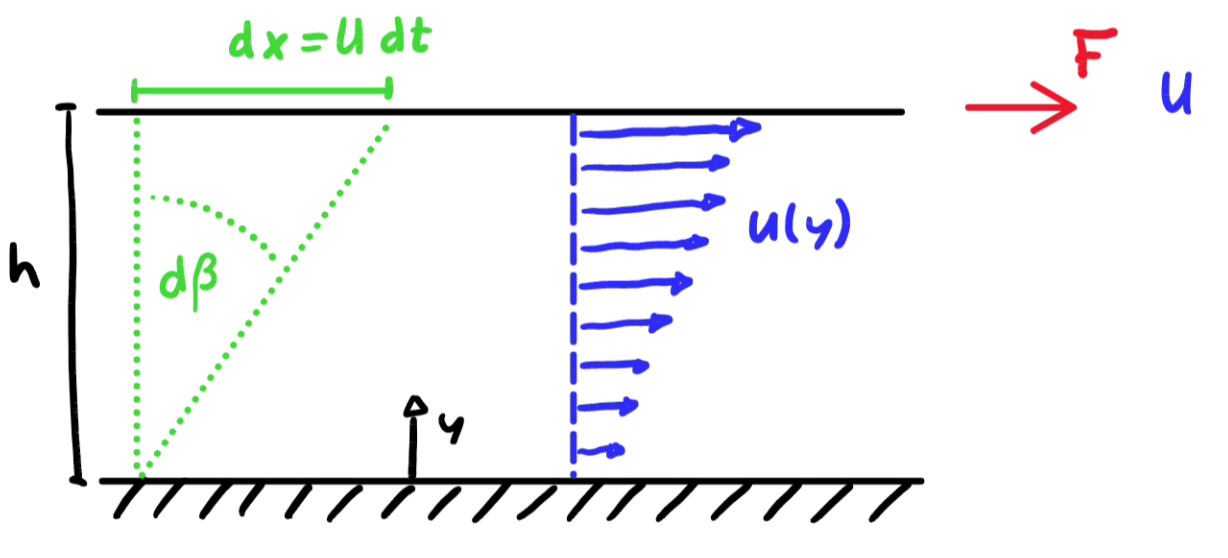
\includegraphics[width=0.4\textwidth]{NoSlip.png}
    \caption{Two plates have a fluid in between. After applying a pure shear force, the top plate moves with velocity $U$. This moves our magically marked atoms on the top by $dx=Udt$.}
    \end{center}
\end{figure}
We can pose the tangent of $d\beta$ to find the deplacement at a height $h$. For small deplacements we can find the change in angle over time to be the \textbf{shear strain rate} $\dot \gamma$
$$
\tan d\beta = \frac {dx}h \approx d\beta \qquad d\beta << 1\implies \frac {d\beta}{dt} = \frac{dx}{hdt}=\frac Uh =: \dot \gamma\qquad [\dot \gamma] = s^{-1}
$$
\paragraph{Notes}
Anywhere in the domain, we can approximate that
$$
\frac Uh \approx\frac {dU}{dy}
$$
\subsection{Newtonian Fluids}
How can we relate the equations of shear stress and shear strain rate? 
We define as \textbf{newtonian fluids} as all the fluids, where the relationship between the applied shear stress is proportional to the shear strain rate (i.e. how much does it respond):
\begin{equation}
\tau = \frac FA \propto \frac {dU}{dy}\implies \tau = \mu \frac{dU}{dy}\label{eq:newtonian_fl}
\end{equation}

\shadowbox{For a newtonian fluid, the more force I apply, the faster it moves (linearly).}
\subsection{Viscosity}

\subsubsection{Dynamic Viscosity}
We define the factor of linearity $\mu$ in \ref{eq:newtonian_fl} to be \textbf{viscosity} (often called dynamic viscosity)
$$
[\mu] = \frac {\mathrm{kg}}{\mathrm m\cdot \mathrm s}
$$

\subsubsection{Kinematic Viscosity}

$$
\nu := \frac \mu \rho\qquad [\nu] =\frac {\mathrm m^2}{s} 
$$
\subsubsection{Notes} 
\begin{itemize}
    \item The stress-strain rate relation in general can be more complex in other flow geometries. But for newtonian fluids it remains linear.
    \item In theory, viscosity $\mu$ is tensor of rank 4. Through symetries, this often collapses to a scalar.
    \item In solids, there are so called Hookean materials which are analogous to Newtonian fluids, where the strain is linear whereas in newtonians the strain rate is linear.
\end{itemize}
\subsubsection{Common Values of Viscosity}
At normal conditions:
\begin{figure}[H]
    \begin{minipage}{0.45\textwidth}
        \centering
        \begin{tabular}{ll}
        \textbf{Material} & \textbf{Viscosity $\mu$ in $\mathrm{kg}/(\mathrm m\cdot \mathrm s)$}\\
        \hline
        Air      & $1.8\cdot 10^{-5}$                         \\
        \hline
        Water    & $1.1\cdot 10^{-3}$                          \\
        \hline
        "Oil"    & $0.4$                       
        \end{tabular}

    \end{minipage}
    \hfill
    \begin{minipage}{0.45\textwidth}
        \centering
        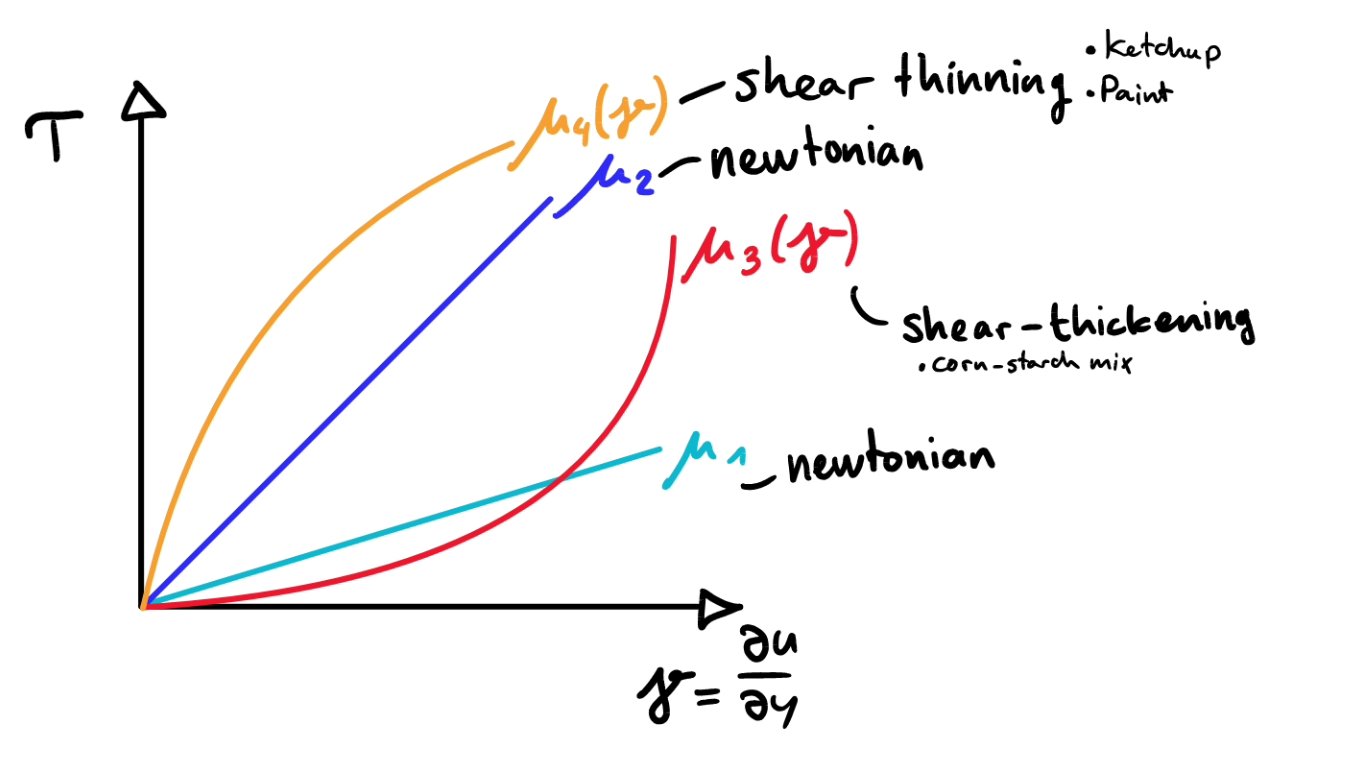
\includegraphics[width=\textwidth]{Newtonian_NonNewtonian.png}

    \end{minipage}
\end{figure}

\paragraph{cgs: Poise}
The poise (only centi-poise is really used) is a commonly used unit for viscosity
$$
\frac{\mathrm g}{\mathrm{cm}\cdot\mathrm s} =: \mathrm{poise} = \mathrm p = 100 \mathrm{cp}
$$

\section{Application: Simple Flow Problem (Munson 1.69)}
We consider the setup in the figure bellow. Two fluids are seperated by an infinite plate at a given height. The top most plate moves at a given velocity $U$. We want to determine the velocity $V$ of the center plate. Additionally we assume that $\mu_2=2\mu_1$.

\begin{figure}[H]
    \begin{minipage}{0.45\textwidth}   
                \centering
            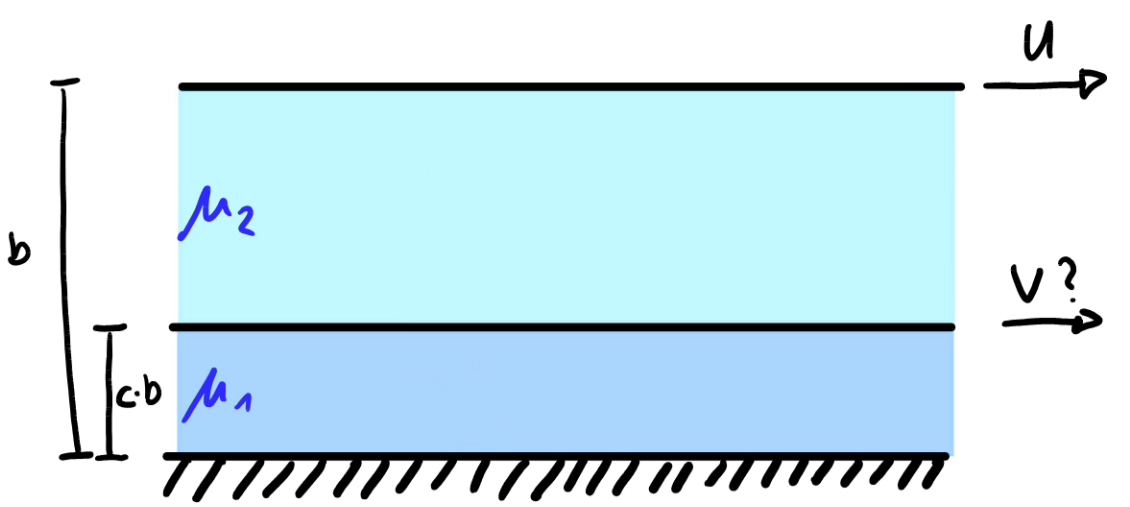
\includegraphics[width=\textwidth]{FlowProblem_1_69a.png}
            \caption{The two fluids with their respective viscosities. The ground plate is fixed and the top moves at a given velocity.}            
    \end{minipage}
    \hfill
    \begin{minipage}{0.45\textwidth}
        \centering
        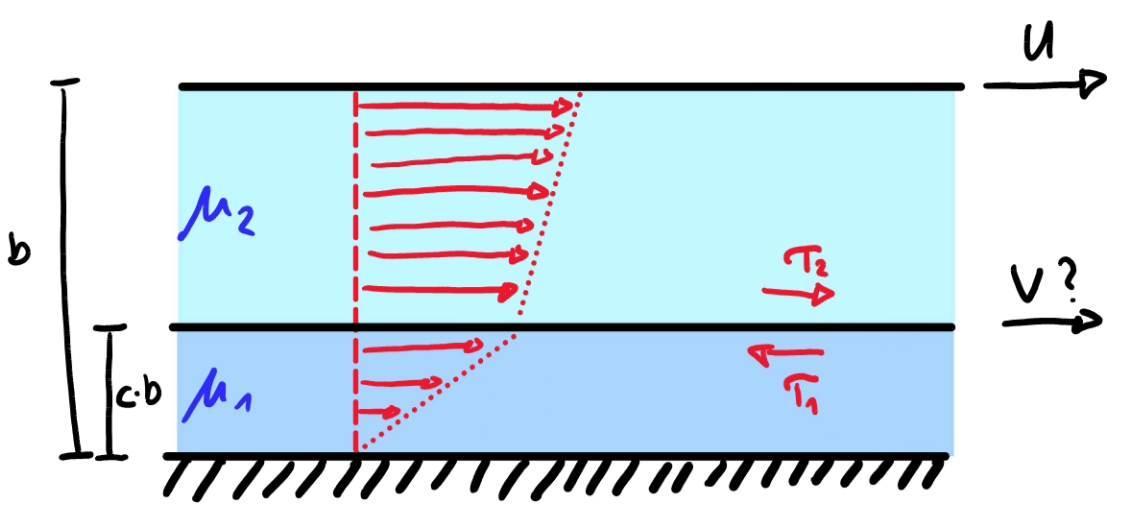
\includegraphics[width=\textwidth]{FlowProblem_1_69b.png}
        \caption{We add shear stresses to the drawing and draw the displacement distribution along the height.}
    \end{minipage}
\end{figure}

We apply the force balance on the middle plate:
\begin{equation*}
    \begin{split}
    \sum F_H = \tau_2A-\tau_1A &\stackrel{*}{=} 0\qquad *: a= 0\\
    \implies \tau_1 &= \tau_2
    \end{split}
\end{equation*}
Expressing $\tau_1$ in terms of variables yields:
$$
\tau_1 = \mu_1\frac V{cb}\stackrel{!}{=}\tau_2=\mu_2\frac{U-V}{(1-c)b}
$$
After solving for $V$ to get:
$$
V=\frac {2c}{1+c}U
$$
To verify boundary conditions, we test for $c=0$ and $c=1$:
$$
\begin{cases}
c=0\implies V=0\\
c=1 \implies V = U
\end{cases}
$$
These results make sense to us.
\chapter{Hydrostatics}
This chapter is based on Munson Chapter 2.

\section{Pressure at a point}
\label{sec:pressure_at_point}
We commonly assume that pressure at a point is a scalar. However, pressure is the component of stress which is normal to a surface.

We consider a wedge-shaped element of fluid. We apply Newton's force balance to the element, for this we need to transform the pressures acting on the surfaces into forces $F_y,F_z,F_s$. Furthermore, we make the assumption that there are no tangential forces on any of the surfaces: we are neglecting all shearing forces.


\begin{figure}[H]
	\centering
	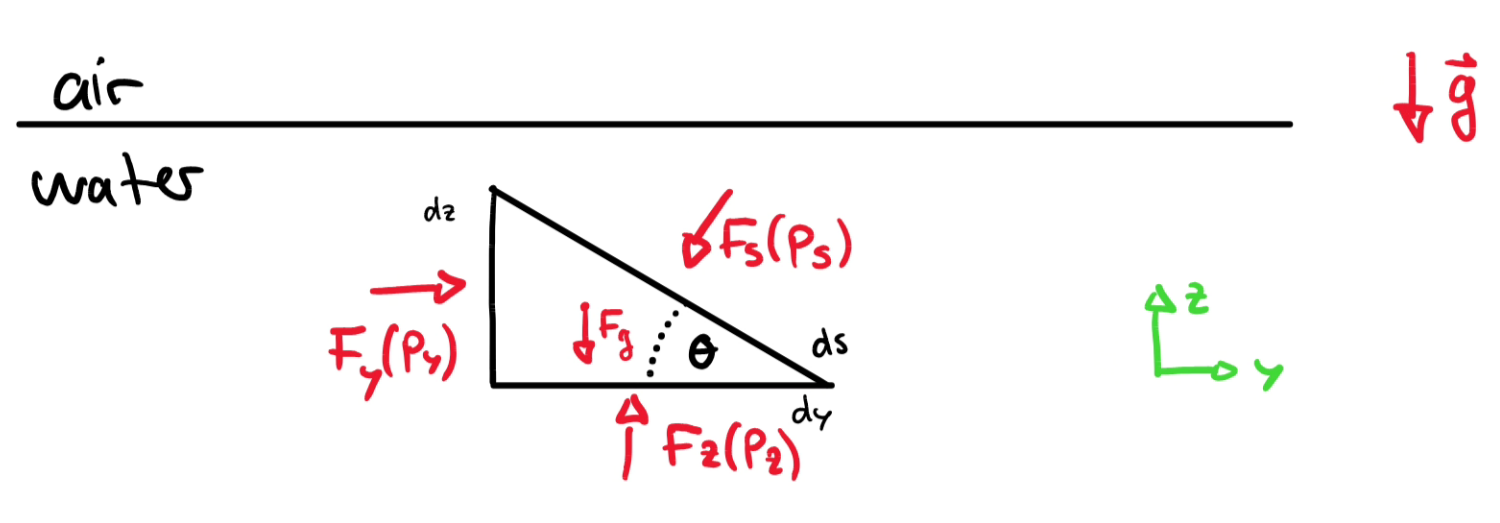
\includegraphics[width=0.6\textwidth]{WedgeElement.png}
	%\caption{}            
\end{figure}

Newton's second law in $z$ direction yields:
\begin{equation*}
	\begin{split}
		\sum \vec F &= m \vec a \\
		\quad F_z = p_z\cdot dx\cdot dy - p_s \cdot ds\cdot dx\cdot \cos \theta-\rho g dV &= \rho dV a_z\qquad \left | \begin{cases}ds = \frac {dy} {\cos\theta}\\ dV = \frac{dz\cdot dy}{2}dx\end{cases}\right.\\
		p_z-p_s -\rho g \frac{dz}2 &= \rho \frac {dz}2a_z\\
		dx,dy,dz\to 0 \implies p_z&=p_s
	\end{split}
\end{equation*}
Similarly we can do the calculation in $x$ and $y$, which results in a final result of
$$
p_z=p_x=p_y=p_s
$$
for any angle $\theta$.

Seeing that the pressure is equal for any direction, we can conclude that $p$ is a scalar
\section{Equation for Pressure Field}
Using the same idea as for \ref{sec:pressure_at_point}, we look at a box.
\begin{figure}[H]
	\centering
	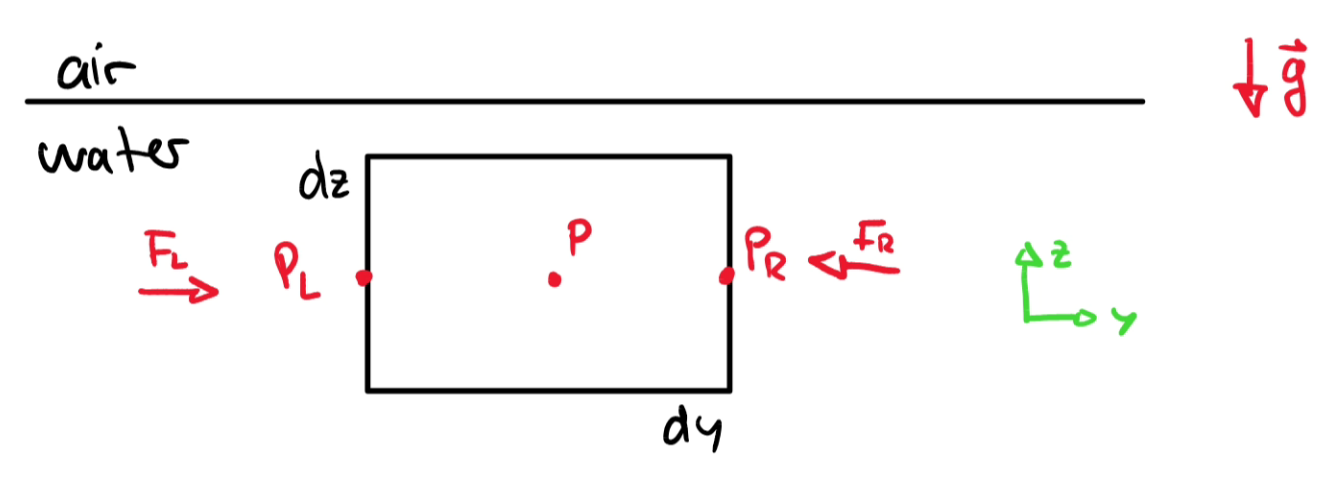
\includegraphics[width=0.6\textwidth]{CubeElement.png}
	%\caption{}            
\end{figure}
We use Taylor expansion to express $p_l$ and $p_r$:
\begin{equation*}
	\begin{split}
		p_r &= p + \left.\frac{dy}{2}\frac{\partial p}{\partial y}\right|_0+\dots\\
		p_l &= p - \left.\frac{dy}{2}\frac{\partial p}{\partial y}\right|_0+\dots\\
		\implies F_R &= p_r\cdot dx\cdot dz = \left( p + \left. \frac{dy}{2}\frac{\partial p}{\partial y}\right|_0\right)dx\cdot dy+\dots\\
		\implies F_L &= p_l\cdot dx\cdot dz = \left( p - \left. \frac{dy}{2}\frac{\partial p}{\partial y}\right|_0\right)dx\cdot dy+\dots\\
	\end{split}
\end{equation*}
We apply force balance in $y$:
\begin{equation*}
	\begin{split}
		-F_R+F_L&=\rho dVa_y\\
		\left.-dy\frac{\partial p}{\partial y}\right|_0\cdot dx\cdot dz &= \rho\cdot dx\cdot dy\cdot dz\cdot a_y+\dots \\
		-\left.\frac{\partial p}{\partial y}\right|_0&=\rho a_y+\dots
		\stackrel{\lim_{dx,dy,dz\to 0 }}{\implies}\left.-\frac{\partial p}{\partial y}\right|_0=\rho a_y
	\end{split}
\end{equation*}
We could do the same calculation in the $x$ and $z$ direction, where the weight needs to be considered. We can rewrite Newtons second law per unit volume:
\begin{equation}
	\boxed{-\nabla p -\rho g\hat k =\rho \vec a}
	\label{eq:newtons_second_law_per_unit_volume}
\end{equation}
\paragraph{Remark} Remember that we neglected shear forces to derive this result. It is only valid if we have no shear forces.

\section{Fluids at Rest}
When a fluid is at rest, from newtons second law we can say that $\vec a = \vec 0$. The derived equation for newton seconds law per unit volume \eqref{eq:newtons_second_law_per_unit_volume} then yields:
\begin{equation}
	\begin{split}
		-\frac{\partial p}{\partial x} &= 0\\
		-\frac{\partial p}{\partial y} &= 0\\
		-\frac{\partial p}{\partial z}-\rho g &= 0
	\end{split}
	\label{eq:fluid_at_rest}
\end{equation}
Which means that the pressure only depends on $z$:
$$
p = p(z)
$$
We can solve the differential equation in \eqref{eq:fluid_at_rest} to find the pressure function explicitly:
\begin{equation}
	\begin{split}
		\frac{\partial p}{\partial z} &= -\rho g\\
		\int dp &= - \int \rho g dz\\
		\Delta p &\stackrel{(*)}{=} - g \int \rho\, dz
	\end{split}
	\label{eq:pressure_difference}
\end{equation}
Where at $(*)$ we assumed the gravitational acceleration to be constant.
\subsection{Incompressible Fluid}
If $\rho$ is constant, a fluid is considered to be an incompressible fluid. The equation for pressure difference \eqref{eq:pressure_difference} is simple to solve:
\begin{equation*}
	\Delta p = -g\rho \Delta z
\end{equation*}
Choosing a coordinate system that goes down with $h$ (height below reference surface) and has its origin such that $h_0=0$ at $p_0$ we can reorder
\begin{equation}
	\boxed{p(h)=\rho g h + p_h}
	\label{eq:pressure_incompressible}
\end{equation}
\paragraph{Remark}
Remember that $p$ is absolute pressure, relative to vacuum. Compared to gage pressure, which is relative to a reference pressure such as the atmospheric pressure. Gage pressure in the above equation \eqref{eq:pressure_incompressible} would be $p-p_h = \rho g h$

\subsection{Compressible Fluid}
To think of compressible fluids (i.e. $d\rho \ne 0$) such as ideal gases, we recall the ideal gas law: $p=\rho R T\implies \rho = p/{RT}$. Combining with the z component of \eqref{eq:fluid_at_rest} we know:
\begin{equation*}
	\begin{split}
		\frac{dp}{dz} &= -\frac{p}{RT}g\\
		\frac 1p \,dp &= -\frac g{RT} dz\qquad (\ast)\\
		\ln(p) &= -\frac g{RT}z + C\\
		p(z) &= C_1\exp\left(-\frac{g}{Rt}z\right)
	\end{split}
\end{equation*}
We assumed at $(\ast)$ that we are at an isothermal atmosphere ($T=const$). To find the integration constant, we pose that at $z=0$ we have a pressure of $p_0$. This yields the \textbf{pressure of ideal gas for isothermal atmosphere}:
\begin{equation}
	\boxed{p(z)=p_0e^{-\frac g{RT}z }}
	\label{eq:pressure_compressible_isothermal}
\end{equation}

Instead of assuming an isothermal atmosphere, we can assume a linear regression of temperature as a function of height, which is accurate up to a certain height (see \ref{fig:temperatureatmosphere}).
\begin{figure}
	\centering
	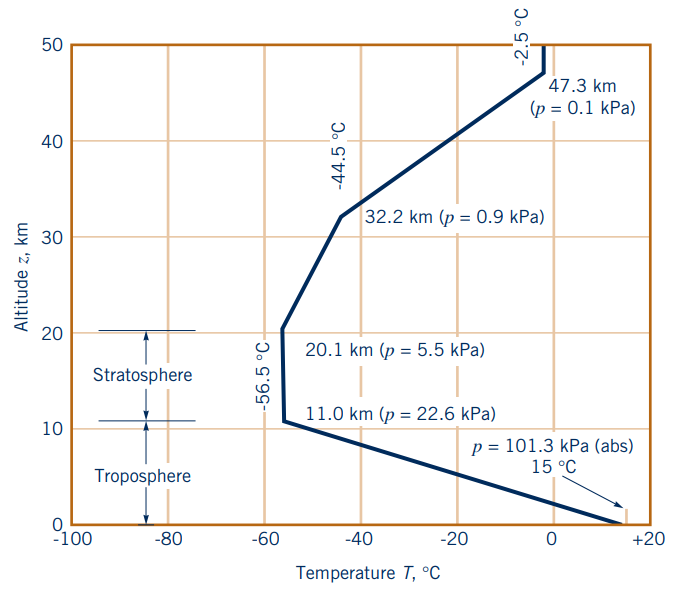
\includegraphics[width=0.4\linewidth]{Sketches/TemperatureAtmosphere}
	\caption{The temperature gradient in our atmosphere (Munson et al, Fluid Dynamics)}
	\label{fig:temperatureatmosphere}
\end{figure}
This leads us, with the \textbf{Standard Atmosphere} of $T(z) = T_0-\beta z$ to the following result of the \textbf{pressure of ideal gas for non-isothermal atmosphere}:
\begin{equation}
	\boxed{p(z)=p_0(1-\frac{\beta z}{T_0})^{\frac{g}{R\beta}}}
\end{equation}


\paragraph{Notes}
The units of pressure are Newton per square-meters, yielding Pascal. $1\ \mathrm{atm}$ is equivalent to $1.01\cdot 10^5\ \mathrm{Pa}$ and $760\ \mathrm{mmHg}$.

\section{Forces on Submerged Surfaces}

\subsection{Flat Surfaces}
\textit{(Munson 2.8)}\hfill\\

We consider a flat surface submerged in an incompressible fluid at an angle $\theta$. 
\begin{figure}[H]
	\centering
	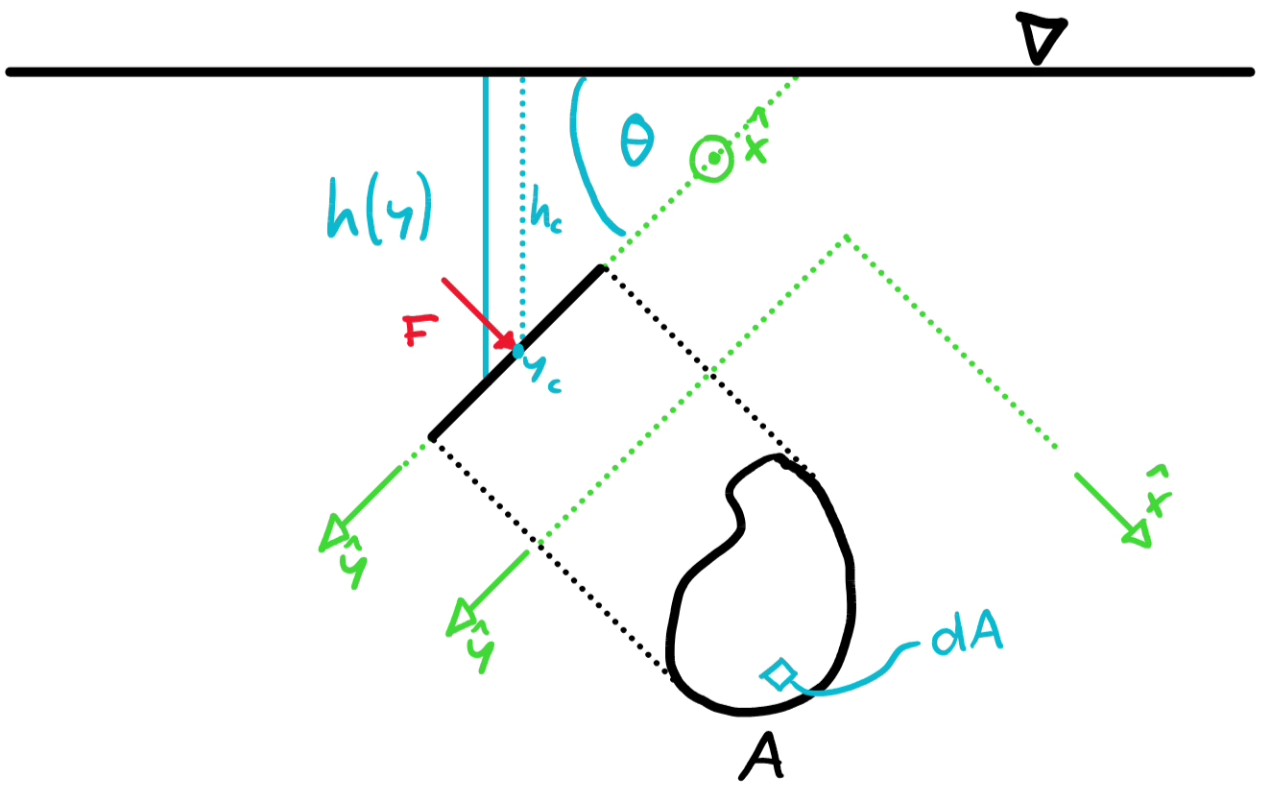
\includegraphics[width=0.5\linewidth]{Sketches/ForceOnFlatSurface}
	\caption{}
	\label{fig:forceonflatsurface}
\end{figure}

We can immediately say:
\begin{equation*}
	p = \rho gh, \qquad h = \sin\theta
\end{equation*}
We integrate over the surface:
\begin{equation*}
	\begin{split}
		F & =\int_A \rho gh \,dA\\
		&=\int_A \rho gy\sin\theta\, dA\\
		&=\rho g \sin\theta \int_A y\, dA\\
		&= \rho g \sin\theta A y_c\\
	\end{split}
\end{equation*}
We recognized the integral as the centroid\footnote{the "average" point, defined as $A^{-1}\int_A y\,dA$. Common values can be found in \ref{fig:geometricalpropertiesshapes}} multiplied by the area at $(\ast)$. Recognizing that $\sin\theta y_c = h_c$, and $\rho g h_c = p_c$. This yields
\begin{equation}
	\boxed{F=p_c A}
\end{equation}
Which makes intuitive sense: The magnitude of the resultant force is given by the pressure at the centroid times the area. It is independent of the orientation ($\theta$ in this case).

To find the point of application of the resultant, we want the distributed force to generate the same moment as the resultant force. We choose the origin of our coordinate system to calculate the moments:
\begin{figure}[H]
	\centering
	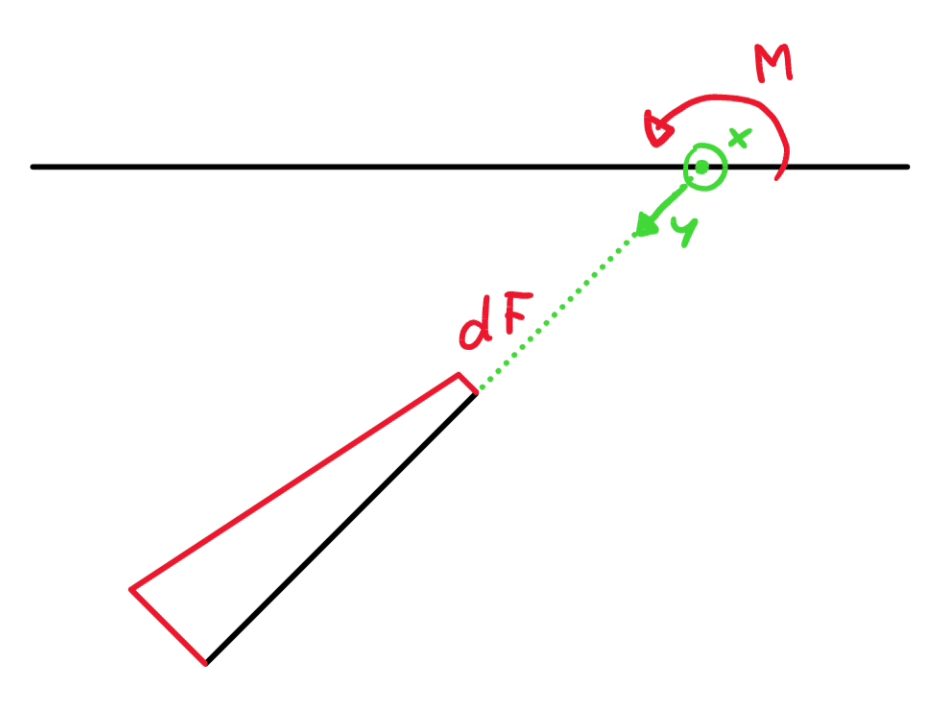
\includegraphics[width=0.5\linewidth]{Sketches/ForceOnFlatSurface_Moment}
	\caption{}
	\label{fig:forceonflatsurfacemoment}
\end{figure}

\begin{equation*}
	\begin{split}
	dF &= \rho gh\,dA = \rho g y\sin\theta dA\\ 
	dM &= y\,dF = \rho\sin\theta y^2\, dA\\
	 M &= \rho g\sin\theta \int_A y^2\, dA\\
	 &= \rho g\sin\theta I_x
	\end{split}
\end{equation*}
Using Steiner's Theorem ($I_x=I_{xc}+Ay_c^2$), we can translate the moment of inertia to the centroid axis and write the final condition for the point of application of the resultant force:
\begin{equation*}
	\begin{split}
		M &= \rho g \sin\theta (I_{xc}+Ay_c^2) = F y_r = \rho g y_c\sin\theta A y_r\\
		\implies &\boxed{y_r = y_c + \frac{I_{xc}}{y_c A }}
	\end{split}
\end{equation*}
From this equation, the application point is always bellow the centroid.


\begin{figure}[H]
	\centering
	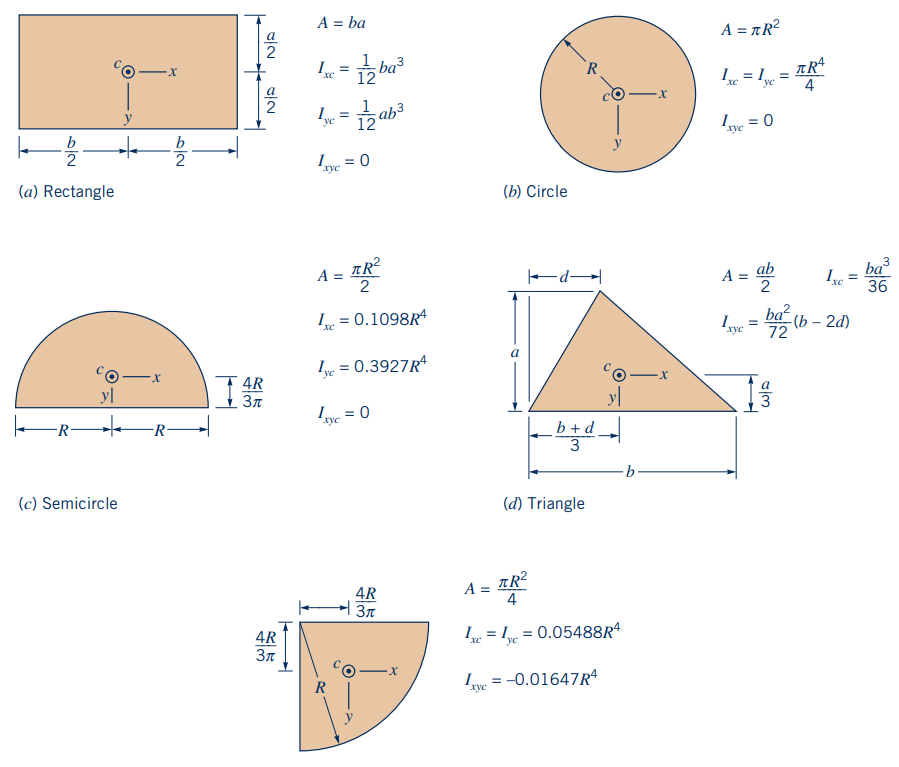
\includegraphics[width=0.7\linewidth]{Sketches/GeometricalPropertiesShapes}
	\caption{Geometrical properties of common shapes (Munson et al, Fluid Dynamics)}
	\label{fig:geometricalpropertiesshapes}
\end{figure}

\subsection{Curved Surfaces}
\textit{(Munson 2.10)}\hfill\\

We decompose the resultant force $\vec F_R$ into its components $\hat i, \hat j$. For both components we integrate over the area, approaching each infinitesimal area $dA$ as a flat surface.

\begin{equation*}
	\begin{split}
		\vec F_R &= F_H\hat i + F_V \hat j\\
		dF &= pdA
	\end{split}
\end{equation*}
Through geometry, we find that $F_H$ is the force acting on the vertical projection of the surface:
\begin{equation*}
	dF_H = pdA\cos\theta = pdA_V\implies F_H=\int pdA_V
\end{equation*}
\begin{figure}[H]
	\centering
	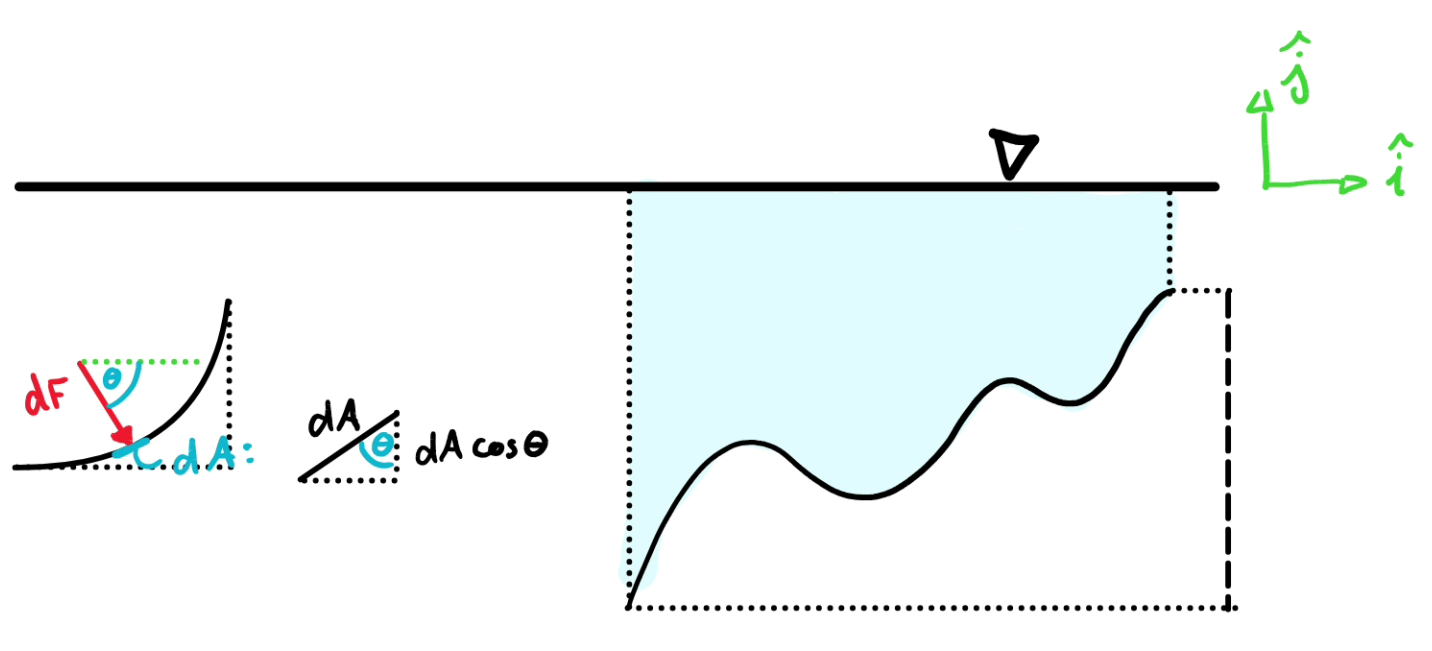
\includegraphics[width=0.7\linewidth]{Sketches/ForceOnCurvedSurface}
	\label{fig:forceoncurvedsurface}
\end{figure}

Similarly, we find that for the vertical component, the force acting vertically on the surface is equal to the weight of the water column above surface:
\begin{equation*}
	dF_V=pdA\sin\theta = \rho ghdA\sin\theta \rho g dV \implies F_V = \int_A g\rho dV 
\end{equation*}


\section{Example Problems}
\subsection{Force on a Tank Sidewall}
Consider a tank sidewall. What is the total resultant force on the surface of the sidewall?
\begin{figure}[H]
	\centering
	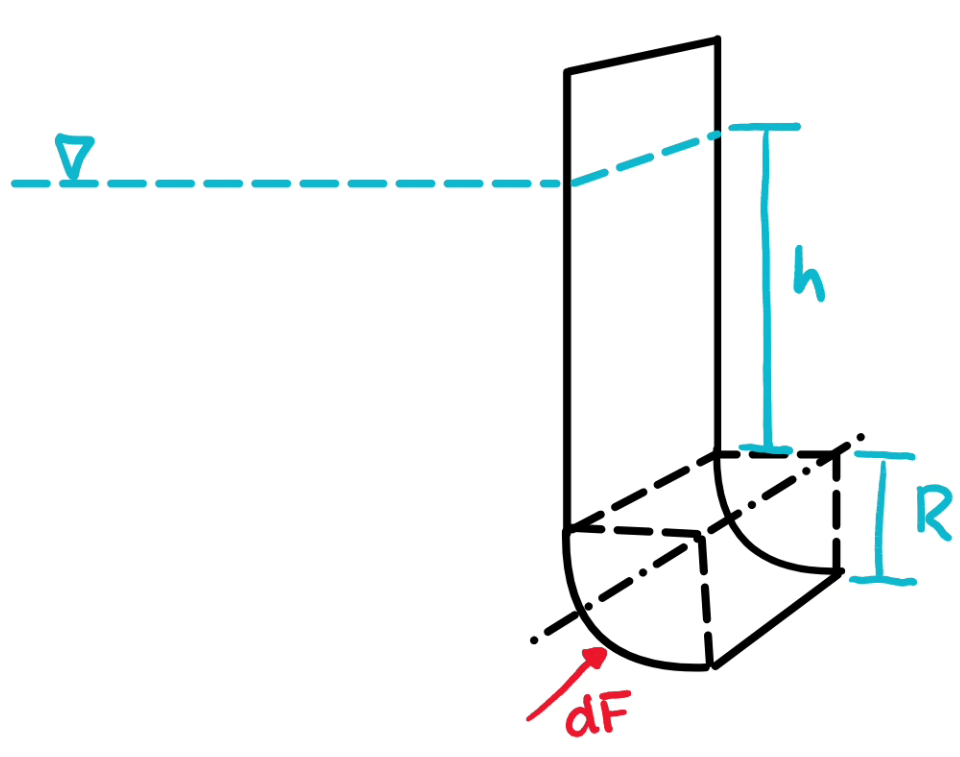
\includegraphics[width=0.4\linewidth]{Sketches/ExampleTankSidewall}
\end{figure}

The vertical component:
\begin{equation*}
	F_V = \int_AdF_V = \left[hRw+\frac{\pi R^2}{4}w\right] \rho g
\end{equation*}
horizontal:
\begin{equation*}
	\begin{split}
		F_H &= \int_A dF_H \\
		&=\text{force on vertical projection} \\
		&= \text{Area * pressure at centroid} \\
		&=  p_cA_V = \rho g\left(h+\frac R2 \right)R_w
	\end{split}
\end{equation*}


\subsection{Archimedes' Principle}
\begin{figure}[H]
	\centering
	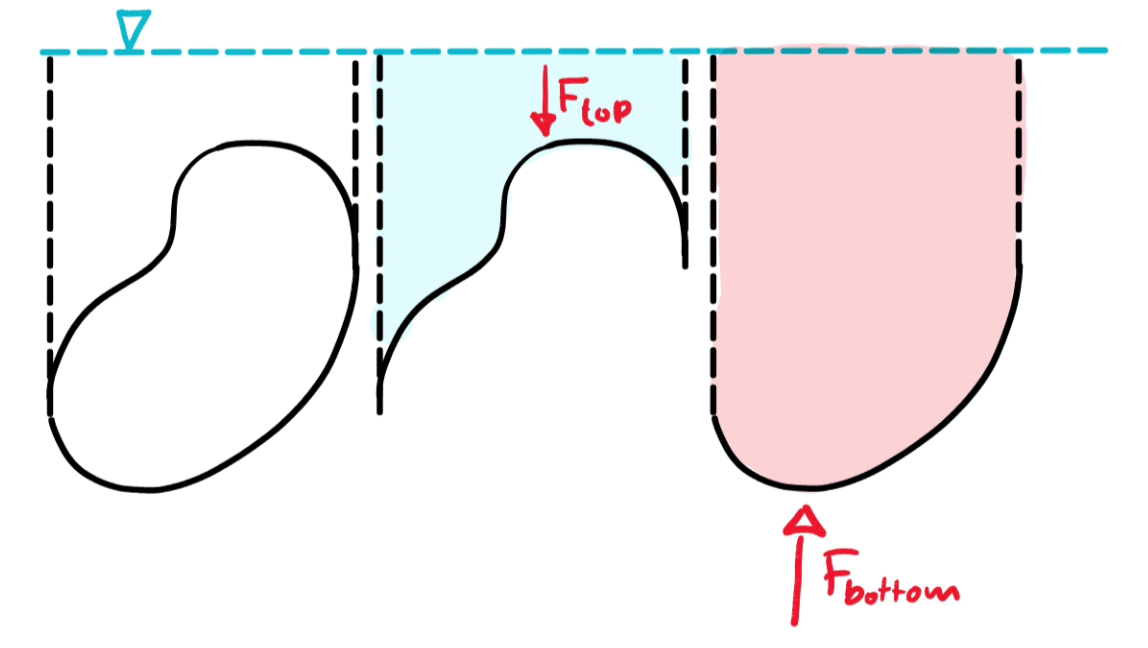
\includegraphics[width=0.7\linewidth]{Sketches/Archimedes}
	\label{fig:archimedes}
\end{figure}
$$
F_{net} = F_{bottom} - F_{top} = \text{weight of the displaced volume}
$$




\chapter{Fluid Dynamics and Bernoulli's Equation}
This chapter is based on Munson Chapter 3.

\section{Definitions}
\paragraph{Streamline (SL)}
Streamlines are lines that are tangent to the velocity vector field at all points in space.

\begin{figure}[H]
	\centering
	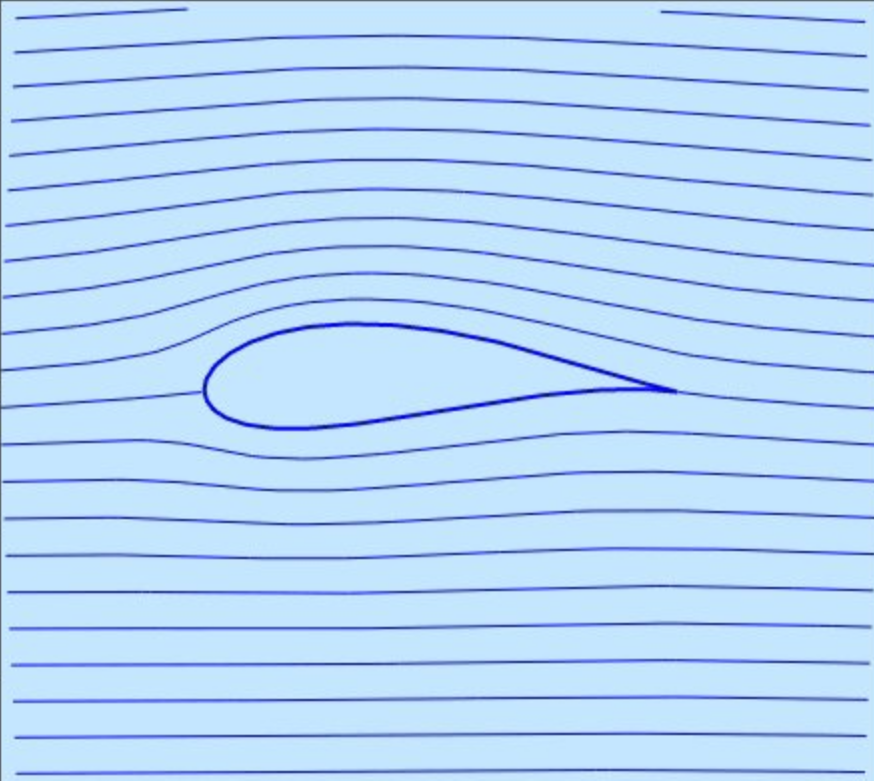
\includegraphics[width=0.3\linewidth]{Sketches/Airfoil}
	\caption{Streamlines along an airfoil}
	\label{fig:airfoil}
\end{figure}

\paragraph{Steady Flow}
When the velocity field $\vec v(\vec r, t)$ is time independent, we call the flow field \textbf{steady}. In this case the stream line is followed by fluid elements.


\section{Derivation of Bernoulli's Equation}

Recall newtons second law per unit volume \eqref{eq:newtons_second_law_per_unit_volume}:
\begin{equation*}
	-\nabla p - \rho g \hat k = \rho \vec a.
\end{equation*}

\begin{figure}[H]
	\centering
	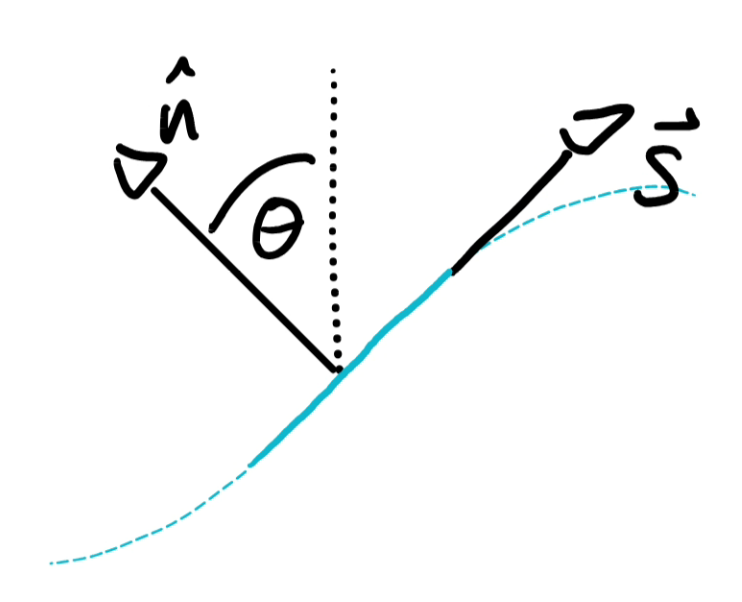
\includegraphics[width=0.3\linewidth]{Sketches/AlongStreamline}
	\caption{Coordinate system setup along a streamline.}
	\label{fig:alongstreamline}
\end{figure}

Along a stream line, (\ref{fig:alongstreamline}) with a normal with an angle $\theta$ to the vertical, we can use \eqref{eq:newtons_second_law_per_unit_volume} to state:


\begin{equation*}
	\begin{split}
		\vec a &= \frac{d\vec v}{dt} = a_s \hat s + a_n \hat n\\
		\text{in s-direction:}\quad a_s &= \frac{\partial v}{\partial s} \frac{\partial s}{\partial t} = \frac{\partial v}{\partial s} v\\
		\implies -\frac{\partial p}{\partial s} - \rho g\sin\theta &= \rho v\frac{\partial v}{\partial s}\\
		-\frac{\partial p}{\partial s} - \rho g \frac{\partial z}{\partial s} &= \rho \frac 12 \frac{\partial (v^2)}{\partial s}\\
		\frac 12 \rho \frac{\partial (v^2)}{\partial s} + \frac{\partial p}{\partial s} + \rho g \frac{\partial s}{\partial s} &= 0
	\end{split}
\end{equation*}

We integrate this along the streamline (in $s$), under the assumption that $\rho$ is constant:
\begin{equation}
	\boxed{\frac 12 \rho v^2 + p + \rho g z = C}
	\label{eq:bernoullis_equation}
\end{equation}
Which is \textbf{Bernoulli's Equation}, with units of energy per unit volume, or pressure. This equation is only valid if:
\begin{itemize}
	\item we have steady flow
	\item $\rho$ is constant
	\item we calculate along one streamline
	\item we can neglect viscosity / we have no shear forces.
\end{itemize}

Its first component ($v^2p/2$) is called \textbf{dynamic pressure}, the second ($p$) is the \textbf{static pressure}, the third ($\rho gz$) is called \textbf{head pressure} or \textbf{elevation pressure}. The first and second term combined is the \textbf{stagnation pressure}

\subsection{Stagnation Streamline}

\begin{figure}[H]
	\centering
	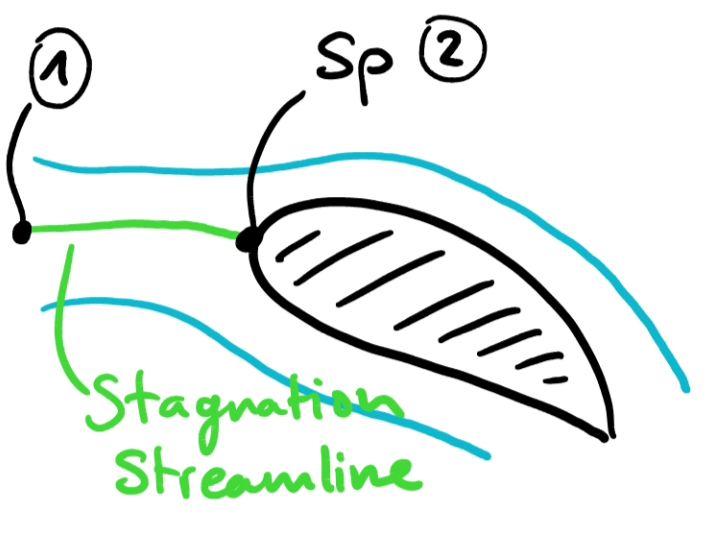
\includegraphics[width=0.3\linewidth]{Sketches/StagnationStreamline}
	\caption{The centred streamline that ends in the \textbf{Stagnation Point} (SP) is called \textbf{Stagnation Streamline}.}
	\label{fig:stagnationstreamline}
\end{figure}
Applying the Bernoulli's Equation for the stagnation streamline, yields:
\begin{equation*}
	p_1+\frac 12\rho v_1^2 = p_2 + \frac 12 \cancel{\rho v_2^2}^{\ast}
\end{equation*}
We ignored the $z$ term, because the pressure differences at flying altitude are negligible compared to the velocity of a plane. We cancel $\ast$ by the observation, that the velocity of the stream at the stagnation point is zero.

\subsection{Newton's 2nd law Across Streamlines}

Recall the coordinate system setup along a streamline (\ref{fig:alongstreamline}). To derive Bernoulli's Equation, we looked in the $s$-direction. If we look in the streamline-normal direction $\hat n$, we arrive at:
\begin{equation*}
	\begin{split}
		-\frac{\partial p}{n}-\rho g \cos \theta &= \rho \frac {v^2}R\qquad \left| \cos \theta= \frac{\partial z}{\partial n}\right.\\
		-\frac {dp}{dn}-\rho g \frac{dz}{dn} = \rho \frac{v^2}R\\
		-dp - \rho g \,dz &= \rho \frac{v^2}R dn
	\end{split}
\end{equation*}
Where $R$ is the \textbf{radius of curvature along $\hat n$}. We integrate the above term across the streamline, in $\hat n$ direction, yielding an important result:
\begin{equation}
		 \boxed{p + \rho gz + \rho \int \frac{v^2}{R}\,dn = C}
\end{equation}
Not knowing $R$ in the most cases makes this result unusable. However, if we have rectilinear (or nearly rectilinear) streamlines, the integration term disappears, as $R \to \infty$. From this we get the much more useable form:
\begin{equation}
	\boxed{p + \rho gz = C}
\end{equation}
\begin{figure}[H]
	\centering
	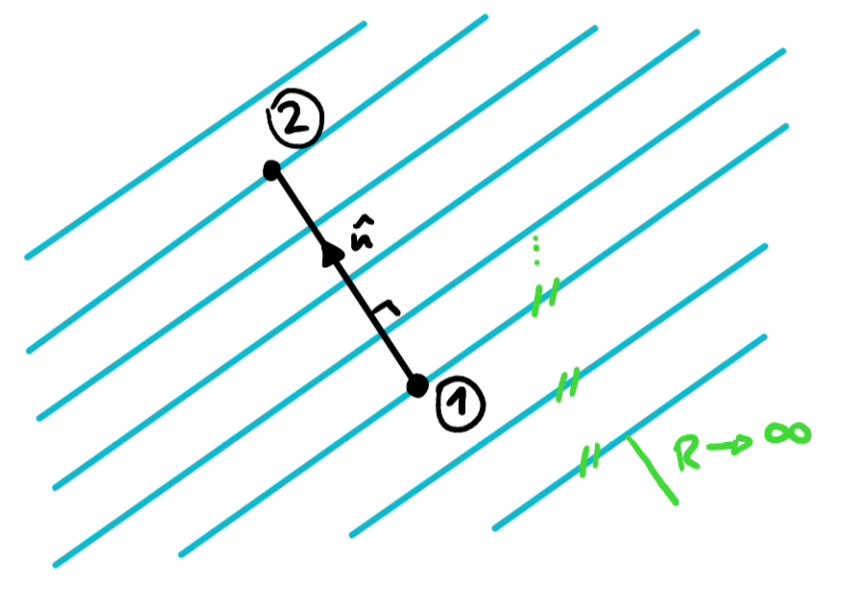
\includegraphics[width=0.4\linewidth]{Sketches/RectilinearStreamLines}
	\caption{All the streamlines are parallel to each other and straight ($R\to \infty$). We can take the difference between two points along the perpendicular direction $\hat n$.}
	\label{fig:rectilinearstreamlines}
\end{figure}
Applying this to a case like \ref{fig:rectilinearstreamlines} yields:
\begin{equation}
	p_2-p_1 = -\rho g (z_2-z_1) \implies p_1 = p_2+\rho gh
\end{equation}
Which can be recognized as one of the laws from hydrostatics.


\section{Applications}
\subsection{Pitot Tube}
To measure the speed with respect to the surrounding air, for example in a plane, pitot tubes are used. It consists of two tubes inside of each other. You can attach a gauge to measure the pressure difference between the two tubes, from which the speed can be found.
\begin{figure}[H]
	\centering
	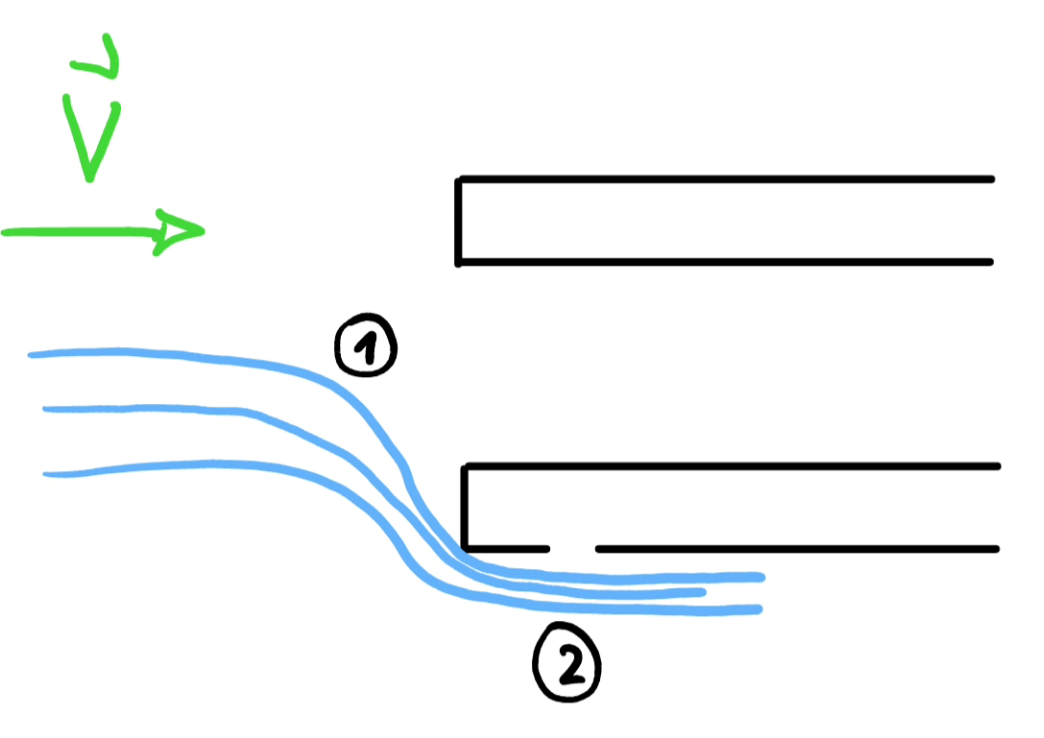
\includegraphics[width=0.4\linewidth]{Sketches/pitot_tube}
	\caption{A simplified representation of a pitot-tube.}
	\label{fig:pitottube}
\end{figure}

We can apply the Bernoulli equation \eqref{eq:bernoullis_equation} while neglecting gravity:
\begin{equation*}
	\frac 12\rho v^2+ p = C
\end{equation*}
Applying this to point 1 yields
\begin{equation*}
	p_1+\frac 12\rho v_1^2 = p+\frac 12 \rho v^2
\end{equation*}
We neglect the velocity difference (therefore $v_1=v$) in order to get the relation $p_1=p$. The measured pressure at point (1) is equal to the environment pressure.

For the second point we say that $v_2=0$ to get
\begin{equation*}
	p_2 = p + \frac 12 \rho v^2 
\end{equation*}

From the above relations we can summarize:
\begin{equation*}
	\begin{split}
		 p_2-p_1&=\frac 12 \rho v^2\\
		 v&=\sqrt{2\frac{p_2-p_1}\rho}
	\end{split}
\end{equation*}
We can conclude that by measuring the difference of pressure we can directly find the air speed.

\subsection{Venturi Tube}
\subsubsection{Mass Conservation and Steady Flow}
Consider a tube with walls that are defined by stream lines. 

\begin{figure}[H]
	\centering
	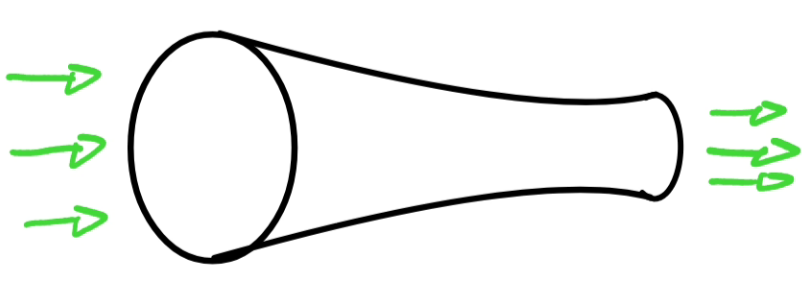
\includegraphics[width=0.4\linewidth]{Sketches/stream_tube}
	\caption{A stream tube: There are no walls, but we know that no mass is flowing through the borders, as they are defined through streamlines}
	\label{fig:streamtube}
\end{figure}

We can define the mass flow rate $\dot m$, where $[\dot m] = \frac{\mathrm{kg}}{\mathrm{s}}$.
and volume flow rate: $\dot V = v A$.
Using conservation of mass we write:
\begin{equation*}
	\rho_1 v_1 A_1 = \rho_2 v_2 A_2
\end{equation*}
for steady flow.

\subsubsection{Application of Mass Conservation}
\begin{figure}[H]
	\centering
	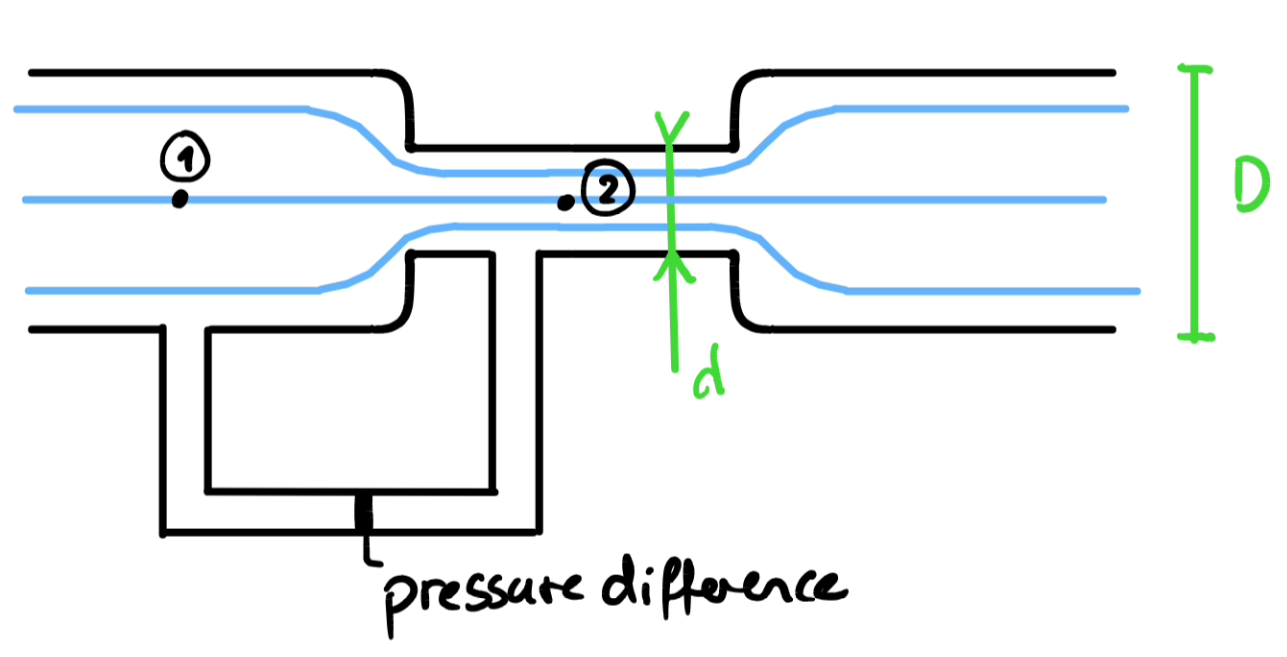
\includegraphics[width=0.7\linewidth]{Sketches/VenturiTube}
	\caption{}
	\label{fig:venturitube}
\end{figure}
We want to find the flow rate of a tube. For this, we add a thinner part and measure the pressure difference between (1) and (2). We apply the Bernoulli equation
\begin{equation*}
	 \frac 12 \rho v_1^2+p_1+\rho gz_1 = \frac 12 \rho v_2^2 + p_2 + \rho gz_2
\end{equation*}
to get the relationship
\begin{equation*}
	v_1^2+ 2 \frac {p_1-p_2}{\rho}=v_2^2
\end{equation*}
We need to apply mass or volume conservation in order to solve this any further, assuming  $\rho  = const$ we get that $v_1D^2 = v_2d^2$ which yields
\begin{equation*}
	v_2 = \sqrt{\frac{2(p_1-p_2)}\rho\div \left(\frac{D^4}{d^4}-1\right)}
\end{equation*}

\subsection{Free Jet}
Consider a bucket filled with a liquid. At the bottom we make a hole and allow the water to flow though.
\begin{figure}[H]
	\centering
	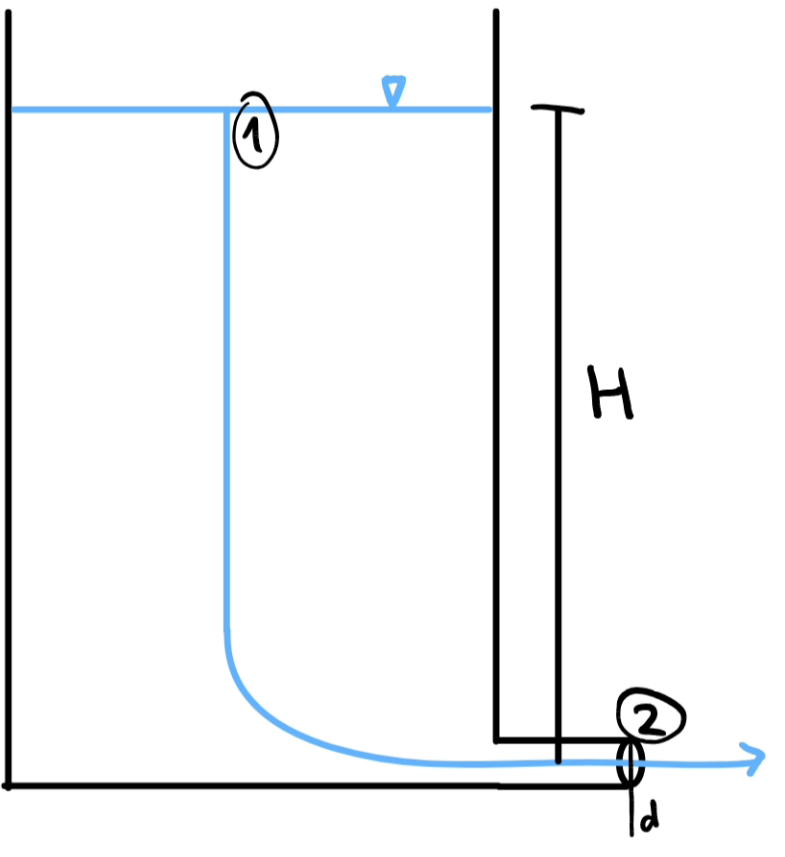
\includegraphics[width=0.3\linewidth]{Sketches/FreeJet}
	\label{fig:freejet}
\end{figure}

We choose a streamline from the centre to avoid shear forces that we would have if we were at the border. We assume that quasi-steady conditions apply (therefore fluid elements follow the same streamlines) for short time intervals or large buckets.

We apply Bernoulli's equation between (1) and (2) to get
\begin{equation*}
	\rho \frac{v_1^2}2+ \rho gz_1 + p_1 = \rho \frac{v_2^2}2+\rho gz_2 + p_2
\end{equation*}

we find that $z_1=H, z_2=0, v_1\approx 0, p_1=p_{atm}, p_2=p_{atm}$ simplifying 
\begin{equation*}
	\rho g H = \rho \frac{v_2^2}{2}\implies v_2^2=\sqrt{2gH}
\end{equation*}
Which is the same result as the speed of a free falling particle after height $H$.

To get the flow rate, we multiply the velocity by the cross-section:
\begin{equation*}
	\dot V = v_2\frac \pi 4 d^2=\frac{\sqrt{2gH}d^2\pi}4
\end{equation*}


\subsubsection{Vena Contracta}
Streamlines cannot abruptly change direction. Therefore the diameter of a stream after a contraption is always smaller or equal to the diameter of the hole:
\begin{figure}[H]
	\centering
	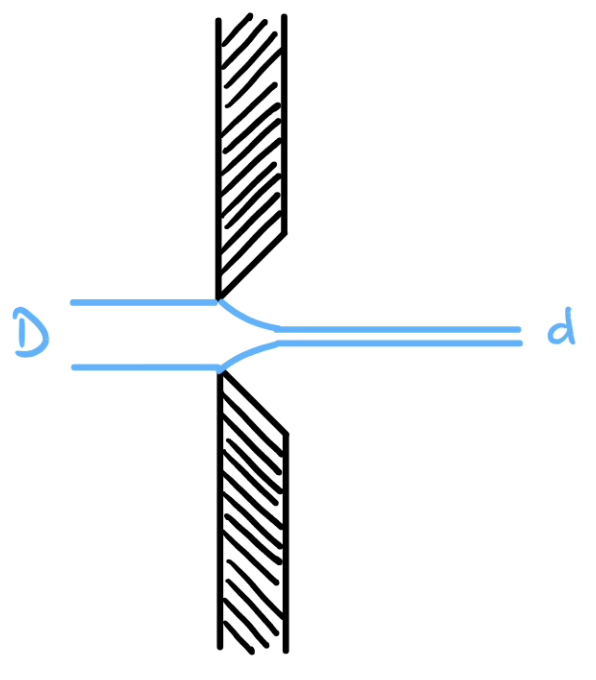
\includegraphics[width=0.3\linewidth]{Sketches/VenaContracta}
	\caption{}
	\label{fig:venacontracta}
\end{figure}
We define the contraction coefficient:
\begin{equation*}
	C_c = \frac{d^2}{D^2}\le 1
\end{equation*}

\setcounter{chapter}{3}
\renewcommand{\thechapter}{D}
\chapter{Diffusion}


\section{Introduction and Diffusion Equation}
We define \textbf{diffusion} as the transport of "stuff" (i.e. small particles, molecules dye, etc.) in a fluid without flow.

\paragraph{Remarks} Diffusion and convection transport often happen simultaneously. Chemical diffusion is a form of mass transport that is mathematically (but not physically) similar to heat conduction.

\subsection{A Microscopic Description of Diffusion}
Model: random walk on a 1D-lattice.
\begin{figure}[H]
	\centering
	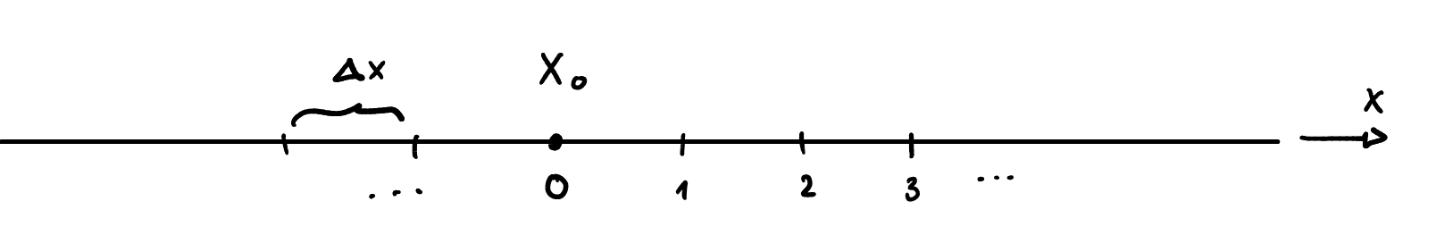
\includegraphics[width=0.7\linewidth]{Sketches/RandomWalk}
	%\caption{}
	\label{fig:randomwalk}
\end{figure}
we call $n(x,t)$ the number of particles at a position $x$ and time $t$ ("number density").

The change of $n$ in a time interval $\Delta t$ can be thought of as follows:

\begin{figure}[H]
	\centering
	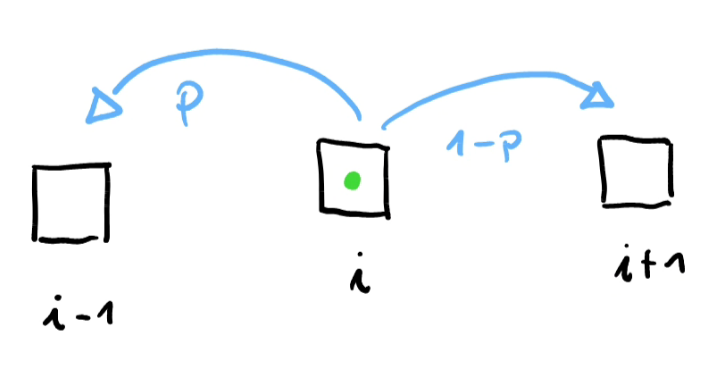
\includegraphics[width=0.3\linewidth]{Sketches/RandomWalkJumps}
	\caption{}
	\label{fig:randomwalkjumps}
\end{figure}

We assume that a particle jumps left with probability $p$ and towards the left with probability $1-p$. If $p=1/2$ we talk about an unbiased walk, when $p\ne 1/2$, it is a biased walk.

The change of particles in a time interval can be expressed as the outflow subtracted from the sum of influxes from the left and right:
\begin{equation}
	\Delta n \approx \frac{\partial n}{\partial t}\Delta t = n(x+\Delta x,t)p + n(x-\Delta x, t)(1-p)-n(x,t)
	\label{eq:diffusion_mass_conservation}
\end{equation}

This expression is just a discrete representation of mass conservation: No particle can get lost, they all have to go somewhere.

We treat $n(x,t)$ as continuous\footnote{Fishy, we know. This can also done by integrating formally to get a jump probability against time.} assuming that $\Delta x$s are really small and the amount of boxes is really large. We can therefore take a Taylor expansion:
\begin{equation*}
	\begin{split}
		n(x+\Delta x,t) = n(x)+\Delta x \frac{\partial n}{\partial x} + \frac{(\Delta x)^2}2 \frac{\partial ^2 n}{\partial x^2} + \dots \\
		n(x-\Delta x,t) = n(x)-\Delta x \frac{\partial n}{\partial x} + \frac{(\Delta x)^2}2 \frac{\partial ^2 n}{\partial x^2} + \dots \\
	\end{split}
\end{equation*}
which can be plugged into the equation \eqref{eq:diffusion_mass_conservation}:
\begin{equation*}
	\begin{split}
		\Delta n  &= \Delta x(p - (1-p))\frac{\partial n}{\partial x} + \frac{(\Delta x)^2}2\frac{\partial^2 n}{\partial x^2}+ \dots\\
		\frac{\partial n}{\partial t} &= -(1-2p)\frac{\Delta x}{\Delta t} \frac{\partial n}{\partial x} + \frac{(\Delta x)^2}{2\Delta t} \frac{\partial ^2 n}{\partial x^2}\qquad \left | \Delta x/ \Delta  t = v \right.\\
		\frac{\partial n}{\partial t} + v \frac{\partial n}{\partial x} &= D\frac{\partial ^2 n}{\partial x^2} \qquad \left | 
		\begin{cases}D = \frac{(\Delta x)^2}{2\Delta t} & \text{diffusion coefficient}\\ v=  (1-2p)\Delta x/\Delta t& \text{drift velocity}\end{cases}
		\right .
	\end{split}
\end{equation*}
For an unbiased random walk we pose $p=0.5$ which cancels the drift velocity. This makes the above turn into the well known \textbf{Diffusion Equation}:
\begin{equation}
	\boxed{\frac{\partial n}{\partial t} = D\frac{\partial ^2 n}{\partial x}}
	\label{eq:diffusion_1d}
\end{equation}
With the diffusion coefficient $D: [D]=m^2/s$

\paragraph{Remarks}
\begin{enumerate}
	\setlength{\itemsep}{-5pt}
	\item The net flux towards the left ($x+\Delta x \to x$) of an unbiased random walk is proportional to the gradient of the concentration $n$: $\frac 12 \Delta x \frac{\partial n}{\partial x} + \dots \propto \frac{\partial n}{\partial x}$.\\
	\item The same model applied for a 3D lattice yields a similar equation:$$\frac{\partial n}{\partial t}\ = D\nabla ^2n,\qquad D = \frac{\delta ^2}{6\Delta t}$$
	\item We can use this model to estimate diffusion coefficients: 
	\subitem Self diffusion: we know the velocity of a particle from statistical thermodynamics and can set $D \approx \frac \delta 6 \left(\frac{2k_b T}{m}\right)^{1/2}\approx 1.5\cdot 10^{-5} cm^2/s$ which is very exact.
	\subitem Suspended particles: A sphere of radius $a$ in a liquid with viscosity $\mu$ has a coefficient $D=\frac{k_BT}{6\pi \mu a}$, which is the Stokes-Einstein relation.
\end{enumerate}



\subsection{A Continuum Description of Diffusion}

We consider a concentration field $c(\vec x,t)$ of units $m^{-3}$. We start with the observation that molecules diffuse from higher to lower concentrations, which is expressed in \textbf{Fick's Law}:
\begin{equation}
	\boxed{\vec j = -D\nabla c}
	\label{eq:ficks_law}
\end{equation}

where $\vec j$ is the number flux: $\frac{1}{\mathrm{time}\cdot \mathrm{area}}$

\begin{figure}[H]
	\centering
	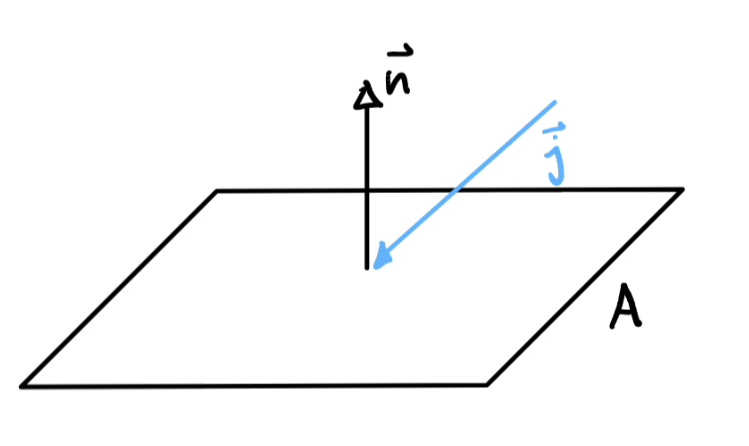
\includegraphics[width=0.3\linewidth]{Sketches/FicksLaw}
	%\caption{}
	\label{fig:fickslaw}
\end{figure}

The number of molecules transported trough area $A$ per time is
\begin{equation*}
	\int_A \vec j \cdot \hat n \, dA
\end{equation*}


Mass conservation in a control volume states, that the rate of change of "stuff" inside is the rate that goes out subtracted from the rate that goes in:
\begin{equation*}
	\begin{split}
	\frac \partial {\partial t}\left[\int_V c\,dV\right] &= -\oint_S \vec j \cdot \,d\vec S\\
	&\stackrel{(*)}{=} \int_V \nabla \cdot \vec j \,dV\\
	\int_V\frac{\partial c}{\partial t}\,dV &= -\int_V \nabla \cdot \vec j \,dV\\
	\int_V\frac{\partial c}{\partial t}- \nabla \cdot \vec j \,dV &= 0\\
	\end{split}
\end{equation*}
where at $(*)$ we used Gauss's law. The volume $V$ is arbitrary, so the above statement is true for all volumes $V$. This is only true, if the integrand is also zero. This leads to a representation of mass conservation in the general form of a differential conservation law:
\begin{equation*}
	\frac{\partial}{\partial t} c + \nabla \cdot \vec j = 0
\end{equation*}

Plugging in Fick's law ($\vec j = -D\nabla c$), we get
\begin{equation*}
	\frac{\partial}{\partial t}c = \nabla (D\nabla c)
\end{equation*}

For $D=const$ we get the \textbf{diffusion equation} from before:
\begin{equation}
	\boxed{\frac{\partial c}{\partial t} = D \nabla^2 c}
\end{equation}

\paragraph{Remarks}

\begin{enumerate}
	\setlength{\itemsep}{-5pt}
	\item The equation results in \eqref{eq:diffusion_1d} in one dimension.
	\item Heat conduction is derived by combining conservation of energy and Fourrier's-Law for chemical energy flux, yielding $\frac{\partial T}{\partial t} = \kappa \nabla ^2 T$ where $\kappa= k/\rho c_p$ is the thermal diffusivity.
	\item The diffusion equation is a partial differential equation (PDE) which needs to be solved with the initial condition (initial concentration) and boundary conditions such as
	\subitem the concentration
	\subitem the flux  $\hat n \cdot \vec j = -D\hat n  \cdot \nabla c$
	\subitem a mix: linked flux with surface concentration (e.g. $\gamma = h(c-c_\infty)$)
\end{enumerate}
 

\section{Solving the Diffusion Equation at Steady State}
\subsection{One Dimensional Linear Problem}
We consider the following system: Two tanks with respective constant concentration $\alpha$ and $\beta$ are connected through a thin pipe of length $l$.
\begin{figure}[H]
	\centering
	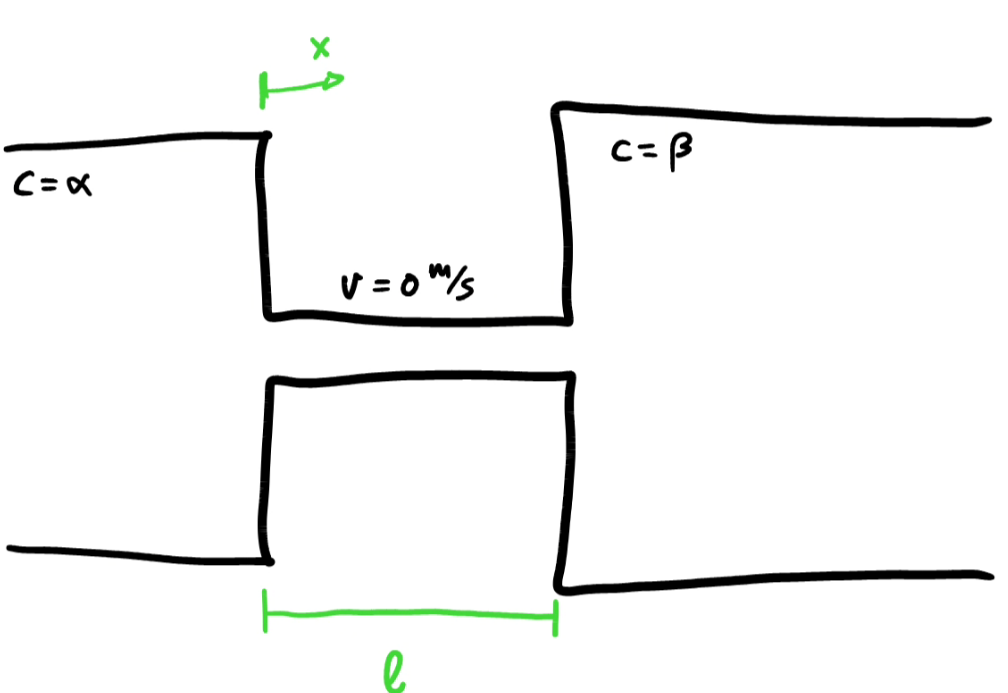
\includegraphics[width=0.5\linewidth]{Sketches/TanksDiffusion}
	%\caption{}
	\label{fig:tanksdiffusion}
\end{figure}

We approximate the pipe as a 1D system, with this we can express the concentration as follows:
\begin{equation*}
	\frac{\partial c}{\partial t} = D\frac{\partial ^2 c}{\partial x^2},\qquad c(x,t),\qquad 0\le 0 \le L
\end{equation*}
We state the boundary conditions:
\begin{equation*}
	\left.\begin{split}
		c(x=0,t)= \alpha\\
		c(x=L,t)= \beta
	\end{split}\right\} \text{Dirichlet Type}
\end{equation*}
At steady state, we know that $\frac{\partial c}{\partial t} = 0$. With these values, there is no initial condition required:
\begin{equation*}
	\begin{split}
		D\frac{\partial ^2 c}{\partial x^2} &= 0\qquad \text{ODE}\\
		c(x) &= A_1x+A_2\\
		\implies &\begin{cases}
			A_1\cdot 0 + A_2 = \alpha\\
			A_1\cdot L + A_2 = \beta
		\end{cases}\\
		c(x) &= \frac{\beta- \alpha}{L}x + \alpha
	\end{split}
\end{equation*}


\paragraph{Notes} The result is unique. It is independent of $D$ because we are assuming steady state, there are no rates.

\subsection{Spherical Problem}

We have two spheres of chemicals and want to find the concentration distribution at steady state.
\begin{figure}[H]
	\centering
	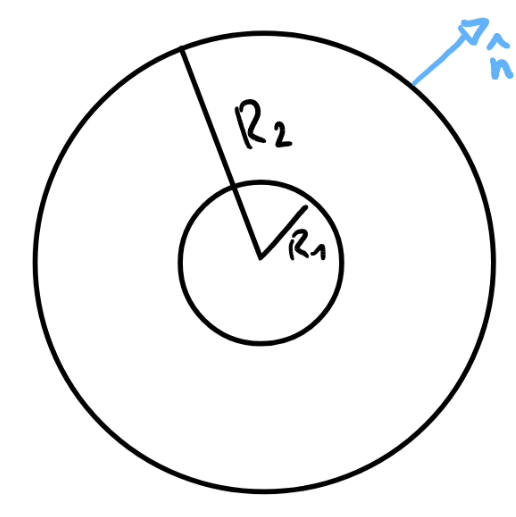
\includegraphics[width=0.4\linewidth]{Sketches/SpheresDiffusion}
	%\caption{}
	\label{fig:spheresdiffusion}
\end{figure}

\begin{equation*}
	\cancel{\frac{\partial c}{\partial t}}^0 = D\nabla ^2 c
\end{equation*}
with the boundary condition of the flux $\vec j \cdot \hat n = -\alpha @ R_2$ and the concentration at $R_1$ is $0$.

If we were to apply the laplacien in cartesian coordinates, we would have difficulties expressing everything, as our system has spherical symmetries, we are better off using the spherical laplacien:
\begin{equation*}
	\nabla^2c = \frac 1{r^2}\frac\partial {\partial r}\left(r^2\frac{\partial c}{\partial r}\right) + \frac 1{r^2\sin\theta}\frac{\partial}{\partial \theta}\left(\sin\theta \frac{\partial c}{\partial \theta}\right) + \frac 1{r^2\sin\theta}\frac{\partial ^2c}{\partial \varphi^2}
\end{equation*}
Through symmetry we know that $c$ is a function of $r$, therefore $\frac{\partial c}{\partial \theta}=\frac{\partial c}{\partial \varphi}=0$. This makes a lot of the terms from the laplacien disappear. What is left is:
\begin{equation*}
	\nabla^2c = \frac 1{r^2}\frac\partial {\partial r}\left(r^2\frac{\partial c}{\partial r}\right)
\end{equation*}
From here we combine the diffusion equation with the laplacien:
\begin{equation*}
	\begin{split}
		0 &= \frac{1}{r^2}\frac{\partial}{\partial r} \left(r^2 \frac{\partial}{\partial r}c\right)\\
		0&=\frac{1}{r^2}\frac{d}{dr}\left(r^2\frac{d}{dr}c\right)\\
		r^2\frac d{dr} c &= A_1\\
		c &= -\frac{A_1}r + A_2\quad
		\begin{cases}
			c(R_1)=0\\
			D\frac{\partial c}{\partial r}\Big|_{R_2} = \alpha\\
			\vec{j} = -D\nabla c
		\end{cases}\\
		\implies & \begin{cases}
		c(r=R_1) = -\frac{A_1}{R_1} + A_2 = 0\\
		D\frac{\partial c}{\partial r}\Big|_{R_2}= D\frac{A_1}{R_2^2}  =\alpha
		\end{cases}\implies \begin{cases}
		A_1=\frac {\alpha R_2^2}{D}\\
		A_2= \frac{\alpha R_2^2}{DR_1}
		\end{cases}\\
		c(r)&=-\frac{\frac {\alpha R_2^2}{D}}{r} + \frac{\alpha R_2^2}{DR_1}\\
		&= \frac{\alpha R_2^2}{D}\left(\frac 1{R_1}-\frac 1{r}\right)
	\end{split}
\end{equation*}

Which looks something like the following plot, plotting for $x\in[R_1,R_2]$:
\begin{figure}[H]
	\centering
	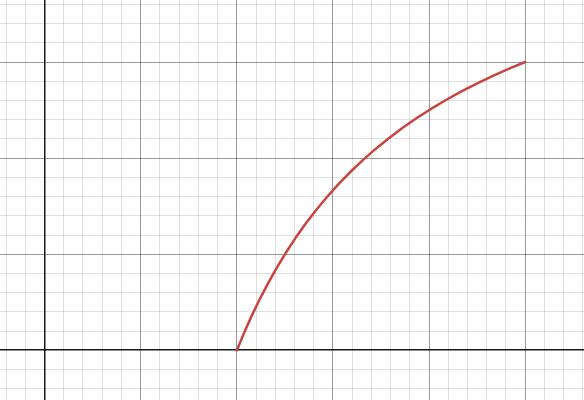
\includegraphics[width=0.4\linewidth]{Sketches/SpheresDiffusionPlot}
	
	\label{fig:spheresdiffusionplot}
\end{figure}

\paragraph{Notes}
This equation is also valid for steady-state with sources and sinks:
\begin{equation*}
	\frac{\partial c}{\partial t} = D \nabla^2c+f
\end{equation*}
where $f$ is for example some chemical reaction ($f=-\alpha$, or $f=-kc$)


\section{Solving the Diffusion Equation with Time Dependency}

\subsection{Finite one Dimensional Domain (Series Expansions)}
\subsubsection{Fixed Concentration}

We pose a partial differential equations the following with boundary conditions and initial conditions:
\begin{equation*}
	\frac{\partial c}{\partial t} = D\frac{\partial^2 c}{\partial x^2}
	\qquad c(x=0,t)=c(x=L,t)=0\qquad c(x,t=0)=c_0(x)
\end{equation*}
Which is a linear and homogenous PDE  with homogeneous boundary conditions.
Therefore if $c_1(x,t)$ and $c_2(x,t)$ are two solutions then $(c_1+c_2)(x,t)$ and $(\beta c_1)(x,t), \beta \in \mathbb R$ are also solutions\footnote{This allows us to look for simple solutions and then construct a sum of the simpler solutions that satisfies the initial conditions.}. Note that this only works for homogeneous boundary conditions. 
The approach is based on linearity: 

\paragraph{Step 1: Write a General Solution} At first, we write a general solution of the PDE with boundary conditions as a linear combination of so-called \textit{base solutions}:
\begin{equation*}
	c(x,t)  = \sum_{n=1}^\infty A_n\varphi_n(x,t)
\end{equation*}
where $\varphi_n$ are simple \textit{base solutions} and $A_n$ are \textit{expansion coefficients}.

\paragraph{Step 2: Determine the Expansion Coefficients} As a second step, we want to determine $\{A_n\}$ such that $c(x,t)$ satisfies the initial condition:
\begin{equation*}
	c(x,t=0)=c_0(x)
\end{equation*}

We start by trying to find any solution, we call \textit{base solution} $\varphi$. We try this by applying separation of variables, assuming $\varphi(x,t)=X(x)T(t)$\footnote{There is no guarantee that we can find a solution of this type. It is an attempt: If I try this, will i find a solution?}. We insert this function into our PDE:
\begin{equation*}
	\begin{split}
		\frac{\partial \varphi}{\partial t} &= D \frac{\partial^2 \varphi}{\partial x^2}\\
		X(x)\frac{dT(t)}{dt}&=DT(t)\frac{d^2 X(x)}{dx^2}\\
		X(x)T'(t)&=DT(t)X''(x)\\
		\frac 1D \frac{T'(t)}{T(t)} &= \frac{X''(x)}{X(x)} \stackrel{(*)}{=}-\lambda\\
	\end{split}
\end{equation*}
Since both sides are independent of each other (left hand side is a function of time, the right hand side is a function of position), it must be equal to a constant $-\lambda$ at $(*)$
The above yields two ordinary differential equations, coupled by an unknown $\lambda$:
\begin{equation*}
		T'(t)+ D\lambda T(t) = 0
		\qquad
		X''(t) + \lambda X(t) = 0
\end{equation*}
The boundary conditions of before still apply:
\begin{equation*}
	\begin{cases}
		\varphi(x=0, t) = 0\\
		\varphi(x=L, t) = 0\\
	\end{cases}\implies
	\begin{cases}
		X(0)=X(L) = 0
	\end{cases}
\end{equation*}
Since the conditions only apply to the spatial equation, we start by solving for $X(t)$, then try to apply our findings to the temporal problem.

We solve $X''(t)+\lambda X(t) = 0$, depending on the sign of $\lambda$ as follows:
\begin{equation*}
	\begin{split}
		\text{Case 1: $\lambda < 0$}: \qquad 
		X(x) & = \alpha_1 e^{{\sqrt-\lambda}x}+ \alpha_2 e^{-\sqrt{-\lambda}x}\\
		 	 & \stackrel{(*)}{=} 0\\
		\text{Case 2: $\lambda = 0$}: \qquad X(x) &= \alpha_1 x + \alpha_2\\
		 	 & \stackrel{(**)}{=} 0\\
		\text{Case 3: $\lambda > 0$}: \qquad X(x) &= \alpha_1 \cos(\sqrt \lambda x) + \alpha_2 \sin(\sqrt \lambda x) \qquad \left | X(0) = 0 \implies \alpha_1 = 0\right .\\
		X(L)&= \alpha_2 \sin(\sqrt \lambda L) = 0\text{ and }\alpha_2 \ne 0\Leftrightarrow \lambda = \left(\frac{\pi n}{L}\right)^2\\
		X(x) &= \alpha_2 \sin\left(\frac{n\pi x}{L}\right)\qquad n \in \mathbb N
	\end{split}
\end{equation*}
At $(*)$ we have reduced the two linearly non-independent solutions and know that $\alpha_1=\alpha_2= 0$, only the trivial solution $X(x)=0$ is found. At $(**)$ we applied the boundary conditions and found the same trivial solution.
An infinite amount of solutions are found for the case where $\lambda > 0$.

Spatial base solutions are those sine/cosine terms which are compatible with the boundary conditions. The boundary conditions determine the coupling constants $\lambda_n$, which we call the eigenvalues of our problem. We now apply this to the temporal problem for a $\lambda_n = \left(\frac{\pi n}{L}\right)^2$:
\begin{equation*}
	\begin{split}
		T_n' &= -D\lambda_n T_n\\
		T_n(T)&=\beta_n e^{-D\lambda_m t} = \beta_n e^{-D\left(\frac{\pi n}{L}\right) ^2 t}
	\end{split}
\end{equation*}
We recognize the solution $T_n$ as a decaying exponential. The combined solution $\varphi$ can be expressed as:
\begin{equation*}
	\varphi_n(x,t) = e^{-D\left(\frac{\pi n}{L}\right) ^2 t} \sin\left(\frac{n\pi x}{L}\right)\qquad n \in \mathbb N\\
\end{equation*}
Through linearity, we were allowed to normalize the solutions and set $\alpha_n \cdot \beta_n = 1$.
The general solution of the PDE that satisfy the boundary conditions can be expressed as:
\begin{equation*}
	c(x,t)= \sum_{n=1}^\infty A_n e^{-D\left(\frac{\pi n}{L}\right) ^2 t} \sin\left(\frac{n\pi x}{L}\right)
\end{equation*}
We now want to determine $\{A_n\}$ from the initial conditions. We need to satisfy:
\begin{equation*}
	c_0(x) = c(x,t=0) = \sum_{n=1}^\infty A_n \sin\left(\frac{n\pi x}{L}\right)
\end{equation*}
Multiplying with one base solution (e.g. $\sin\frac{\pi mx}{L}$ with some integer $m$) and then integrate in $x$:
\begin{equation*}
	\begin{split}
		\int_0^L c_0(x)\sin\left(\frac{\pi m}{L}x \right) \,dx &= \sum_{n=1}^\infty A_n\int_0^L\sin\left(\frac{\pi n}{L} x \right)\sin\left(\frac{\pi m}{L} x \right)\,dx\\
		&\stackrel{(*)}{=}  \sum_{n=1}^\infty A_n\begin{cases}
			0 & n\ne m\\
			L/2 & n=m
		\end{cases}\\
		& = A_n \frac L2\\
		A_n & =\frac 2L \int_0^L c_0(x)\sin\left(\frac{\pi_n}Lx\right)\,dx
	\end{split}
\end{equation*}
At $(*)$ we use the fact that the integral over a common multiple of a period of two sines or cosines with different frequencies yields 0. \footnote{This can be shown using the identity $\sin a \sin b = \frac 12(\cos(a-b)-\cos(a+b))$ over a full period.}

Through Fourier's theorems, we know that any smooth initial condition satisfying my boundary conditions can be expressed as a sine, cosine or Fourier series, meaning we have the complete solution. For any $c_0(x)$, the complete solution is:
\begin{equation}
	\boxed{c(x,t) = \sum_{n=1}^\infty \underbrace{\left[ \frac 2L \int_0^L c_0(\tilde  x)\sin\left(\frac{\pi n}L\tilde x\right)\,d\tilde x\right]}_{\text{expansion coefficient of mode}} \underbrace{e^{-D\left(\frac{\pi n}{L}\right)^2x}}_{\text{time evolution}}\underbrace{\sin\left(\frac{\pi n}{L} x\right)}_{\text{spatial mode}}}
\end{equation}

\subsubsection{Non-Homogeneous Boundary Conditions}
If we want to solve the diffusion equation with non homogenous boundary conditions:
\begin{equation*}
	\frac{\partial c}{\partial t} = D\frac{\partial ^2 c}{\partial x^2}\qquad \begin{cases}
		c(x=0,t) = c_1& \text{boundary condition}\\
		c(x=L,t) = c_2& \text{boundary condition}\\
		c(x,t=0) = c_0(x) & \text{initial condition}
	\end{cases}
\end{equation*}
Similarly to the previous approach, we use multiple steps:

\paragraph{Step A: Solve for Steady State} Let $c_f$ be the final concentration field:
\begin{equation*}
	c_f(x)=\lim_{t\to \infty} = c(x,t)
\end{equation*}
We know how to solve this, applying the boundary conditions of the problem:
\begin{equation*}
	0=\frac{\partial }{\partial t} c_f = D\frac{\partial ^2 c_f}{\partial x^2}\stackrel{\text{BC}}{\implies}c_f(x) = c_1 + \frac{c_2-c_1}{L}x
\end{equation*}

\paragraph{Step B: Finding a Transient Solution $\tilde c$}
We define $\tilde c$ as a superposition / linear combination of the unknown solution $c$ and the known final position $c_f$:
\begin{equation*}
	\tilde c(x,t) := c(x,t) - c_f(x)
\end{equation*}

From this we know that $\tilde c$ will satisfy the diffusion equation. Furthermore, the boundary conditions for $\tilde c$ turn into:
\begin{equation*}
	\frac{\partial \tilde c}{\partial t} = D\frac{\partial ^2 \tilde c}{\partial t^2}\implies\begin{cases}
		\tilde c(x=0) = c(x=0)-c_f(x=0)=c_1-c_1=0\\
		\tilde c(x=L) = c(x=L)-c_f(x=L)=c_2-c_2=0\\
	\end{cases}
\end{equation*}

\paragraph{Step C: Combine}
From the definition of $\tilde c$, we know that 
\begin{equation*}
	c(x,t) = c_f(x) + \tilde c(x,t)
\end{equation*}
Plugging in the transient solution for $\tilde c$ and the final solution $c_f$ will yield the final form for $c(x,t)$.

\setcounter{chapter}{3}
\renewcommand{\thechapter}{\arabic{chapter}}



\setcounter{chapter}{3}
\renewcommand{\thechapter}{D}
\chapter{Diffusion}


\section{Introduction and Diffusion Equation}
We define \textbf{diffusion} as the transport of "stuff" (i.e. small particles, molecules dye, etc.) in a fluid without flow.

\paragraph{Remarks} Diffusion and convection transport often happen simultaneously. Chemical diffusion is a form of mass transport that is mathematically (but not physically) similar to heat conduction.

\subsection{A Microscopic Description of Diffusion}
Model: random walk on a 1D-lattice.
\begin{figure}[H]
	\centering
	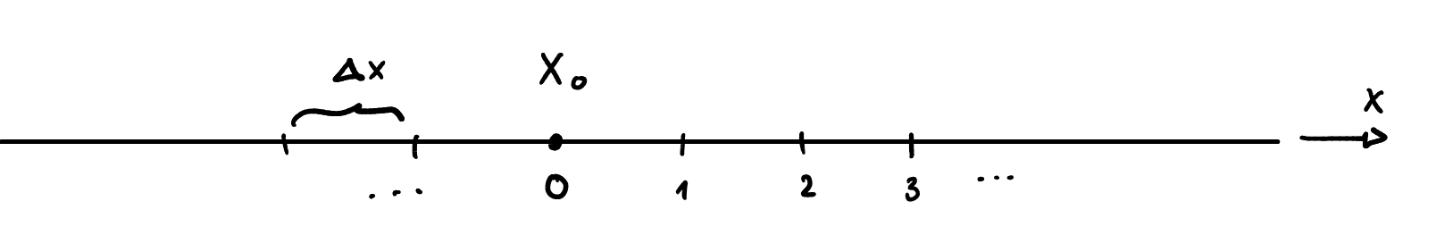
\includegraphics[width=0.7\linewidth]{Sketches/RandomWalk}
	%\caption{}
	\label{fig:randomwalk}
\end{figure}
we call $n(x,t)$ the number of particles at a position $x$ and time $t$ ("number density").

The change of $n$ in a time interval $\Delta t$ can be thought of as follows:

\begin{figure}[H]
	\centering
	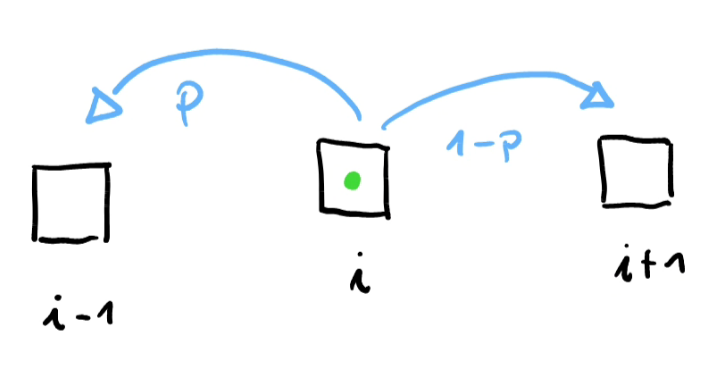
\includegraphics[width=0.3\linewidth]{Sketches/RandomWalkJumps}
	\caption{}
	\label{fig:randomwalkjumps}
\end{figure}

We assume that a particle jumps left with probability $p$ and towards the left with probability $1-p$. If $p=1/2$ we talk about an unbiased walk, when $p\ne 1/2$, it is a biased walk.

The change of particles in a time interval can be expressed as the outflow subtracted from the sum of influxes from the left and right:
\begin{equation}
	\Delta n \approx \frac{\partial n}{\partial t}\Delta t = n(x+\Delta x,t)p + n(x-\Delta x, t)(1-p)-n(x,t)
	\label{eq:diffusion_mass_conservation}
\end{equation}

This expression is just a discrete representation of mass conservation: No particle can get lost, they all have to go somewhere.

We treat $n(x,t)$ as continuous\footnote{Fishy, we know. This can also done by integrating formally to get a jump probability against time.} assuming that $\Delta x$s are really small and the amount of boxes is really large. We can therefore take a Taylor expansion:
\begin{equation*}
	\begin{split}
		n(x+\Delta x,t) = n(x)+\Delta x \frac{\partial n}{\partial x} + \frac{(\Delta x)^2}2 \frac{\partial ^2 n}{\partial x^2} + \dots \\
		n(x-\Delta x,t) = n(x)-\Delta x \frac{\partial n}{\partial x} + \frac{(\Delta x)^2}2 \frac{\partial ^2 n}{\partial x^2} + \dots \\
	\end{split}
\end{equation*}
which can be plugged into the equation \eqref{eq:diffusion_mass_conservation}:
\begin{equation*}
	\begin{split}
		\Delta n  &= \Delta x(p - (1-p))\frac{\partial n}{\partial x} + \frac{(\Delta x)^2}2\frac{\partial^2 n}{\partial x^2}+ \dots\\
		\frac{\partial n}{\partial t} &= -(1-2p)\frac{\Delta x}{\Delta t} \frac{\partial n}{\partial x} + \frac{(\Delta x)^2}{2\Delta t} \frac{\partial ^2 n}{\partial x^2}\qquad \left | \Delta x/ \Delta  t = v \right.\\
		\frac{\partial n}{\partial t} + v \frac{\partial n}{\partial x} &= D\frac{\partial ^2 n}{\partial x^2} \qquad \left | 
		\begin{cases}D = \frac{(\Delta x)^2}{2\Delta t} & \text{diffusion coefficient}\\ v=  (1-2p)\Delta x/\Delta t& \text{drift velocity}\end{cases}
		\right .
	\end{split}
\end{equation*}
For an unbiased random walk we pose $p=0.5$ which cancels the drift velocity. This makes the above turn into the well known \textbf{Diffusion Equation}:
\begin{equation}
	\boxed{\frac{\partial n}{\partial t} = D\frac{\partial ^2 n}{\partial x}}
	\label{eq:diffusion_1d}
\end{equation}
With the diffusion coefficient $D: [D]=m^2/s$

\paragraph{Remarks}
\begin{enumerate}
	\setlength{\itemsep}{-5pt}
	\item The net flux towards the left ($x+\Delta x \to x$) of an unbiased random walk is proportional to the gradient of the concentration $n$: $\frac 12 \Delta x \frac{\partial n}{\partial x} + \dots \propto \frac{\partial n}{\partial x}$.\\
	\item The same model applied for a 3D lattice yields a similar equation:$$\frac{\partial n}{\partial t}\ = D\nabla ^2n,\qquad D = \frac{\delta ^2}{6\Delta t}$$
	\item We can use this model to estimate diffusion coefficients: 
	\subitem Self diffusion: we know the velocity of a particle from statistical thermodynamics and can set $D \approx \frac \delta 6 \left(\frac{2k_b T}{m}\right)^{1/2}\approx 1.5\cdot 10^{-5} cm^2/s$ which is very exact.
	\subitem Suspended particles: A sphere of radius $a$ in a liquid with viscosity $\mu$ has a coefficient $D=\frac{k_BT}{6\pi \mu a}$, which is the Stokes-Einstein relation.
\end{enumerate}



\subsection{A Continuum Description of Diffusion}

We consider a concentration field $c(\vec x,t)$ of units $m^{-3}$. We start with the observation that molecules diffuse from higher to lower concentrations, which is expressed in \textbf{Fick's Law}:
\begin{equation}
	\boxed{\vec j = -D\nabla c}
	\label{eq:ficks_law}
\end{equation}

where $\vec j$ is the number flux: $\frac{1}{\mathrm{time}\cdot \mathrm{area}}$

\begin{figure}[H]
	\centering
	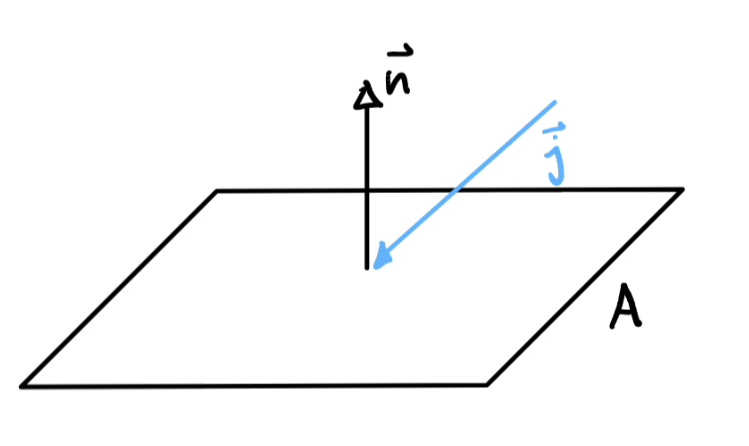
\includegraphics[width=0.3\linewidth]{Sketches/FicksLaw}
	%\caption{}
	\label{fig:fickslaw}
\end{figure}

The number of molecules transported trough area $A$ per time is
\begin{equation*}
	\int_A \vec j \cdot \hat n \, dA
\end{equation*}


Mass conservation in a control volume states, that the rate of change of "stuff" inside is the rate that goes out subtracted from the rate that goes in:
\begin{equation*}
	\begin{split}
	\frac \partial {\partial t}\left[\int_V c\,dV\right] &= -\oint_S \vec j \cdot \,d\vec S\\
	&\stackrel{(*)}{=} \int_V \nabla \cdot \vec j \,dV\\
	\int_V\frac{\partial c}{\partial t}\,dV &= -\int_V \nabla \cdot \vec j \,dV\\
	\int_V\frac{\partial c}{\partial t}- \nabla \cdot \vec j \,dV &= 0\\
	\end{split}
\end{equation*}
where at $(*)$ we used Gauss's law. The volume $V$ is arbitrary, so the above statement is true for all volumes $V$. This is only true, if the integrand is also zero. This leads to a representation of mass conservation in the general form of a differential conservation law:
\begin{equation*}
	\frac{\partial}{\partial t} c + \nabla \cdot \vec j = 0
\end{equation*}

Plugging in Fick's law ($\vec j = -D\nabla c$), we get
\begin{equation*}
	\frac{\partial}{\partial t}c = \nabla (D\nabla c)
\end{equation*}

For $D=const$ we get the \textbf{diffusion equation} from before:
\begin{equation}
	\boxed{\frac{\partial c}{\partial t} = D \nabla^2 c}
\end{equation}

\paragraph{Remarks}

\begin{enumerate}
	\setlength{\itemsep}{-5pt}
	\item The equation results in \eqref{eq:diffusion_1d} in one dimension.
	\item Heat conduction is derived by combining conservation of energy and Fourrier's-Law for chemical energy flux, yielding $\frac{\partial T}{\partial t} = \kappa \nabla ^2 T$ where $\kappa= k/\rho c_p$ is the thermal diffusivity.
	\item The diffusion equation is a partial differential equation (PDE) which needs to be solved with the initial condition (initial concentration) and boundary conditions such as
	\subitem the concentration
	\subitem the flux  $\hat n \cdot \vec j = -D\hat n  \cdot \nabla c$
	\subitem a mix: linked flux with surface concentration (e.g. $\gamma = h(c-c_\infty)$)
\end{enumerate}
 

\section{Solving the Diffusion Equation at Steady State}
\subsection{One Dimensional Linear Problem}
We consider the following system: Two tanks with respective constant concentration $\alpha$ and $\beta$ are connected through a thin pipe of length $l$.
\begin{figure}[H]
	\centering
	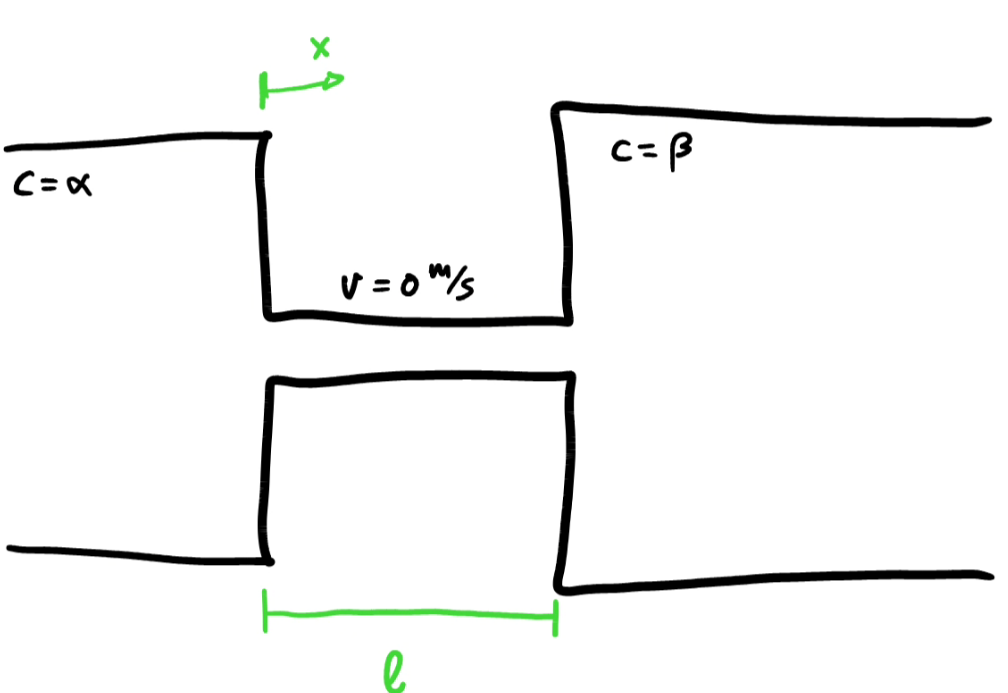
\includegraphics[width=0.5\linewidth]{Sketches/TanksDiffusion}
	%\caption{}
	\label{fig:tanksdiffusion}
\end{figure}

We approximate the pipe as a 1D system, with this we can express the concentration as follows:
\begin{equation*}
	\frac{\partial c}{\partial t} = D\frac{\partial ^2 c}{\partial x^2},\qquad c(x,t),\qquad 0\le 0 \le L
\end{equation*}
We state the boundary conditions:
\begin{equation*}
	\left.\begin{split}
		c(x=0,t)= \alpha\\
		c(x=L,t)= \beta
	\end{split}\right\} \text{Dirichlet Type}
\end{equation*}
At steady state, we know that $\frac{\partial c}{\partial t} = 0$. With these values, there is no initial condition required:
\begin{equation*}
	\begin{split}
		D\frac{\partial ^2 c}{\partial x^2} &= 0\qquad \text{ODE}\\
		c(x) &= A_1x+A_2\\
		\implies &\begin{cases}
			A_1\cdot 0 + A_2 = \alpha\\
			A_1\cdot L + A_2 = \beta
		\end{cases}\\
		c(x) &= \frac{\beta- \alpha}{L}x + \alpha
	\end{split}
\end{equation*}


\paragraph{Notes} The result is unique. It is independent of $D$ because we are assuming steady state, there are no rates.

\subsection{Spherical Problem}

We have two spheres of chemicals and want to find the concentration distribution at steady state.
\begin{figure}[H]
	\centering
	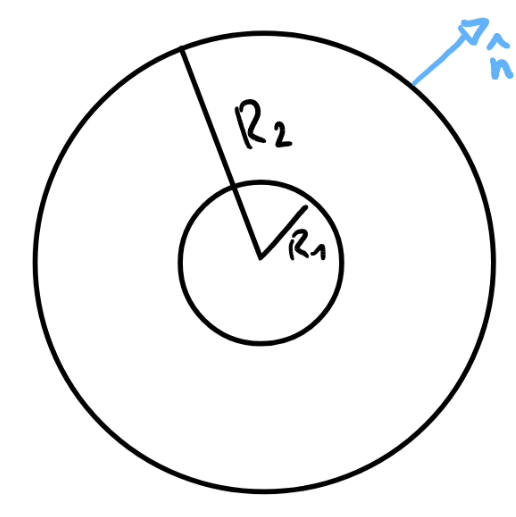
\includegraphics[width=0.4\linewidth]{Sketches/SpheresDiffusion}
	%\caption{}
	\label{fig:spheresdiffusion}
\end{figure}

\begin{equation*}
	\cancel{\frac{\partial c}{\partial t}}^0 = D\nabla ^2 c
\end{equation*}
with the boundary condition of the flux $\vec j \cdot \hat n = -\alpha @ R_2$ and the concentration at $R_1$ is $0$.

If we were to apply the laplacien in cartesian coordinates, we would have difficulties expressing everything, as our system has spherical symmetries, we are better off using the spherical laplacien:
\begin{equation*}
	\nabla^2c = \frac 1{r^2}\frac\partial {\partial r}\left(r^2\frac{\partial c}{\partial r}\right) + \frac 1{r^2\sin\theta}\frac{\partial}{\partial \theta}\left(\sin\theta \frac{\partial c}{\partial \theta}\right) + \frac 1{r^2\sin\theta}\frac{\partial ^2c}{\partial \varphi^2}
\end{equation*}
Through symmetry we know that $c$ is a function of $r$, therefore $\frac{\partial c}{\partial \theta}=\frac{\partial c}{\partial \varphi}=0$. This makes a lot of the terms from the laplacien disappear. What is left is:
\begin{equation*}
	\nabla^2c = \frac 1{r^2}\frac\partial {\partial r}\left(r^2\frac{\partial c}{\partial r}\right)
\end{equation*}
From here we combine the diffusion equation with the laplacien:
\begin{equation*}
	\begin{split}
		0 &= \frac{1}{r^2}\frac{\partial}{\partial r} \left(r^2 \frac{\partial}{\partial r}c\right)\\
		0&=\frac{1}{r^2}\frac{d}{dr}\left(r^2\frac{d}{dr}c\right)\\
		r^2\frac d{dr} c &= A_1\\
		c &= -\frac{A_1}r + A_2\quad
		\begin{cases}
			c(R_1)=0\\
			D\frac{\partial c}{\partial r}\Big|_{R_2} = \alpha\\
			\vec{j} = -D\nabla c
		\end{cases}\\
		\implies & \begin{cases}
		c(r=R_1) = -\frac{A_1}{R_1} + A_2 = 0\\
		D\frac{\partial c}{\partial r}\Big|_{R_2}= D\frac{A_1}{R_2^2}  =\alpha
		\end{cases}\implies \begin{cases}
		A_1=\frac {\alpha R_2^2}{D}\\
		A_2= \frac{\alpha R_2^2}{DR_1}
		\end{cases}\\
		c(r)&=-\frac{\frac {\alpha R_2^2}{D}}{r} + \frac{\alpha R_2^2}{DR_1}\\
		&= \frac{\alpha R_2^2}{D}\left(\frac 1{R_1}-\frac 1{r}\right)
	\end{split}
\end{equation*}

Which looks something like the following plot, plotting for $x\in[R_1,R_2]$:
\begin{figure}[H]
	\centering
	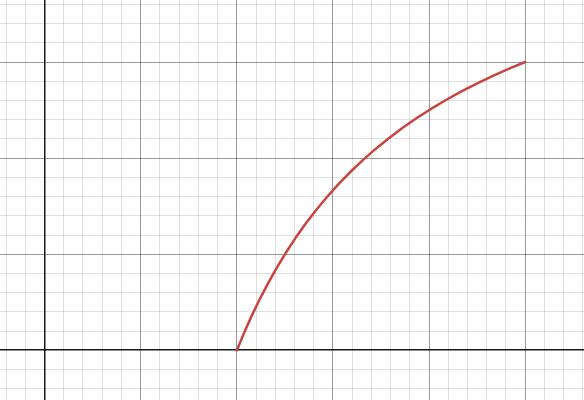
\includegraphics[width=0.4\linewidth]{Sketches/SpheresDiffusionPlot}
	
	\label{fig:spheresdiffusionplot}
\end{figure}

\paragraph{Notes}
This equation is also valid for steady-state with sources and sinks:
\begin{equation*}
	\frac{\partial c}{\partial t} = D \nabla^2c+f
\end{equation*}
where $f$ is for example some chemical reaction ($f=-\alpha$, or $f=-kc$)


\section{Solving the Diffusion Equation with Time Dependency}

\subsection{Finite one Dimensional Domain (Series Expansions)}
\subsubsection{Fixed Concentration}

We pose a partial differential equations the following with boundary conditions and initial conditions:
\begin{equation*}
	\frac{\partial c}{\partial t} = D\frac{\partial^2 c}{\partial x^2}
	\qquad c(x=0,t)=c(x=L,t)=0\qquad c(x,t=0)=c_0(x)
\end{equation*}
Which is a linear and homogenous PDE  with homogeneous boundary conditions.
Therefore if $c_1(x,t)$ and $c_2(x,t)$ are two solutions then $(c_1+c_2)(x,t)$ and $(\beta c_1)(x,t), \beta \in \mathbb R$ are also solutions\footnote{This allows us to look for simple solutions and then construct a sum of the simpler solutions that satisfies the initial conditions.}. Note that this only works for homogeneous boundary conditions. 
The approach is based on linearity: 

\paragraph{Step 1: Write a General Solution} At first, we write a general solution of the PDE with boundary conditions as a linear combination of so-called \textit{base solutions}:
\begin{equation*}
	c(x,t)  = \sum_{n=1}^\infty A_n\varphi_n(x,t)
\end{equation*}
where $\varphi_n$ are simple \textit{base solutions} and $A_n$ are \textit{expansion coefficients}.

\paragraph{Step 2: Determine the Expansion Coefficients} As a second step, we want to determine $\{A_n\}$ such that $c(x,t)$ satisfies the initial condition:
\begin{equation*}
	c(x,t=0)=c_0(x)
\end{equation*}

We start by trying to find any solution, we call \textit{base solution} $\varphi$. We try this by applying separation of variables, assuming $\varphi(x,t)=X(x)T(t)$\footnote{There is no guarantee that we can find a solution of this type. It is an attempt: If I try this, will i find a solution?}. We insert this function into our PDE:
\begin{equation*}
	\begin{split}
		\frac{\partial \varphi}{\partial t} &= D \frac{\partial^2 \varphi}{\partial x^2}\\
		X(x)\frac{dT(t)}{dt}&=DT(t)\frac{d^2 X(x)}{dx^2}\\
		X(x)T'(t)&=DT(t)X''(x)\\
		\frac 1D \frac{T'(t)}{T(t)} &= \frac{X''(x)}{X(x)} \stackrel{(*)}{=}-\lambda\\
	\end{split}
\end{equation*}
Since both sides are independent of each other (left hand side is a function of time, the right hand side is a function of position), it must be equal to a constant $-\lambda$ at $(*)$
The above yields two ordinary differential equations, coupled by an unknown $\lambda$:
\begin{equation*}
		T'(t)+ D\lambda T(t) = 0
		\qquad
		X''(t) + \lambda X(t) = 0
\end{equation*}
The boundary conditions of before still apply:
\begin{equation*}
	\begin{cases}
		\varphi(x=0, t) = 0\\
		\varphi(x=L, t) = 0\\
	\end{cases}\implies
	\begin{cases}
		X(0)=X(L) = 0
	\end{cases}
\end{equation*}
Since the conditions only apply to the spatial equation, we start by solving for $X(t)$, then try to apply our findings to the temporal problem.

We solve $X''(t)+\lambda X(t) = 0$, depending on the sign of $\lambda$ as follows:
\begin{equation*}
	\begin{split}
		\text{Case 1: $\lambda < 0$}: \qquad 
		X(x) & = \alpha_1 e^{{\sqrt-\lambda}x}+ \alpha_2 e^{-\sqrt{-\lambda}x}\\
		 	 & \stackrel{(*)}{=} 0\\
		\text{Case 2: $\lambda = 0$}: \qquad X(x) &= \alpha_1 x + \alpha_2\\
		 	 & \stackrel{(**)}{=} 0\\
		\text{Case 3: $\lambda > 0$}: \qquad X(x) &= \alpha_1 \cos(\sqrt \lambda x) + \alpha_2 \sin(\sqrt \lambda x) \qquad \left | X(0) = 0 \implies \alpha_1 = 0\right .\\
		X(L)&= \alpha_2 \sin(\sqrt \lambda L) = 0\text{ and }\alpha_2 \ne 0\Leftrightarrow \lambda = \left(\frac{\pi n}{L}\right)^2\\
		X(x) &= \alpha_2 \sin\left(\frac{n\pi x}{L}\right)\qquad n \in \mathbb N
	\end{split}
\end{equation*}
At $(*)$ we have reduced the two linearly non-independent solutions and know that $\alpha_1=\alpha_2= 0$, only the trivial solution $X(x)=0$ is found. At $(**)$ we applied the boundary conditions and found the same trivial solution.
An infinite amount of solutions are found for the case where $\lambda > 0$.

Spatial base solutions are those sine/cosine terms which are compatible with the boundary conditions. The boundary conditions determine the coupling constants $\lambda_n$, which we call the eigenvalues of our problem. We now apply this to the temporal problem for a $\lambda_n = \left(\frac{\pi n}{L}\right)^2$:
\begin{equation*}
	\begin{split}
		T_n' &= -D\lambda_n T_n\\
		T_n(T)&=\beta_n e^{-D\lambda_m t} = \beta_n e^{-D\left(\frac{\pi n}{L}\right) ^2 t}
	\end{split}
\end{equation*}
We recognize the solution $T_n$ as a decaying exponential. The combined solution $\varphi$ can be expressed as:
\begin{equation*}
	\varphi_n(x,t) = e^{-D\left(\frac{\pi n}{L}\right) ^2 t} \sin\left(\frac{n\pi x}{L}\right)\qquad n \in \mathbb N\\
\end{equation*}
Through linearity, we were allowed to normalize the solutions and set $\alpha_n \cdot \beta_n = 1$.
The general solution of the PDE that satisfy the boundary conditions can be expressed as:
\begin{equation*}
	c(x,t)= \sum_{n=1}^\infty A_n e^{-D\left(\frac{\pi n}{L}\right) ^2 t} \sin\left(\frac{n\pi x}{L}\right)
\end{equation*}
We now want to determine $\{A_n\}$ from the initial conditions. We need to satisfy:
\begin{equation*}
	c_0(x) = c(x,t=0) = \sum_{n=1}^\infty A_n \sin\left(\frac{n\pi x}{L}\right)
\end{equation*}
Multiplying with one base solution (e.g. $\sin\frac{\pi mx}{L}$ with some integer $m$) and then integrate in $x$:
\begin{equation*}
	\begin{split}
		\int_0^L c_0(x)\sin\left(\frac{\pi m}{L}x \right) \,dx &= \sum_{n=1}^\infty A_n\int_0^L\sin\left(\frac{\pi n}{L} x \right)\sin\left(\frac{\pi m}{L} x \right)\,dx\\
		&\stackrel{(*)}{=}  \sum_{n=1}^\infty A_n\begin{cases}
			0 & n\ne m\\
			L/2 & n=m
		\end{cases}\\
		& = A_n \frac L2\\
		A_n & =\frac 2L \int_0^L c_0(x)\sin\left(\frac{\pi_n}Lx\right)\,dx
	\end{split}
\end{equation*}
At $(*)$ we use the fact that the integral over a common multiple of a period of two sines or cosines with different frequencies yields 0. \footnote{This can be shown using the identity $\sin a \sin b = \frac 12(\cos(a-b)-\cos(a+b))$ over a full period.}

Through Fourier's theorems, we know that any smooth initial condition satisfying my boundary conditions can be expressed as a sine, cosine or Fourier series, meaning we have the complete solution. For any $c_0(x)$, the complete solution is:
\begin{equation}
	\boxed{c(x,t) = \sum_{n=1}^\infty \underbrace{\left[ \frac 2L \int_0^L c_0(\tilde  x)\sin\left(\frac{\pi n}L\tilde x\right)\,d\tilde x\right]}_{\text{expansion coefficient of mode}} \underbrace{e^{-D\left(\frac{\pi n}{L}\right)^2x}}_{\text{time evolution}}\underbrace{\sin\left(\frac{\pi n}{L} x\right)}_{\text{spatial mode}}}
\end{equation}
\setcounter{chapter}{4}
\renewcommand{\thechapter}{\arabic{chapter}}



\chapter{Control Volume Approach using RTT}

Recall the three principal physical laws:
\begin{itemize}
	\setlength{\itemsep}{-5pt}
	\item Mass conservation
	\item Newton's \nth2 law
	\item energy conservation
\end{itemize}
These are all expressed on systems, but we would like to apply them for control volumes. We can use RTT eq. \eqref{eq:rtt_final} to do this.

\section{Mass Conservation}
For mass conservation, the arbitrary quantity $B$ in the RTT is the mass $M$. This implies that $b=1$. We plug $B=M$ into eq. \eqref{eq:rtt_final} and find:
\begin{equation}
	\begin{split}
		\frac{dM_{sys}}{Dt} = \boxed{\frac{\partial}{\partial t}  \int_{cv} \rho dV + \int _{cs} \rho \vec v \cdot \hat n \,dA =0}\\
	\end{split}
	\label{eq:continuity}
\end{equation}
Which is the continuity equation. In words, this means:
\begin{equation*}
	\left(\substack{
		\text{The rate of change}\\
		\text{of the mass in the}\\
		\text{coincident system}
		}\right) = \left(\substack{
		\text{The rate of change}\\
		\text{in the coincident}\\
		\text{control volume}
		}\right) + \left(\substack{
		\text{The net rate of flow}\\
		\text{of mass through}\\
		\text{the control surface}
		}\right)
\end{equation*}

\section{Momentum: Newton's \nth{2} Law}
To express Newton's second law for control volumes, the quantity $\vec B=M\cdot \vec v$. We can think of the vectorised version as a combination of three quantities. $\vec b = \vec v$.
Newton second law in Lagrangian form is:
\begin{equation*}
	\frac{D}{Dt}(M\vec v)_{sys} = \sum \vec F_{sys}
\end{equation*}

We can rewrite the first term into Eularian:
\begin{equation}
\frac{D}{Dt}(M\vec v)_{sys} =\boxed{\frac{\partial}{\partial t}\int_{cv}\rho\vec v \,dV+ \int_{cs}\rho\vec v(\vec v\cdot \hat n)\,dA=\sum \vec F_{\substack{\text{content of the}\\\text{coincident CV}}}}
\end{equation}

If the flow is steady, the first integral is zero.


The integral over the control surface can be decomposed when mass-flow occurs only through a certain number of surfaces. If an area is flat (hence $\hat n=const$), velocity and density are unified, the integral multiplies the area, and we end up with
\begin{equation*}
	\int_A \rho\vec v(\vec v\cdot \hat n)\,dA = \dot M\vec v
\end{equation*}

For steady one-inlet, one-outlet uniform flow problems, we get:
\begin{equation*}
	\sum\vec F = \dot M(\vec v_2-\vec v_1)
\end{equation*}

We can interpret the first term as the \textbf{rate of change of linear momentum in the control volume}, and the right term as side as the \textbf{flux of linear momentum though the control surface}.


\textbf{Note} The control volume must be fixed, non-deforming, and attached to an inertial frame of reference. 


\section{Energy Conservation (\nth{1} Law of Thermodynamics)}

\subsection{General Situation}
We choose $B=E$, the total energy, therefore $b=\frac EM=e$ the total specific energy. The total energy accounts for: internal, kinetic, and potential  energy:
\begin{equation*}
	e=\tilde u+\frac 12 v^2+gz\qquad \vec g = -g\hat k
\end{equation*}
For the Lagrangian system:
\begin{equation*}
	\frac{D}{Dt}\int_{sys}e\rho\,dV = \dot Q_{net, in}+\dot W_{net, in}
\end{equation*}
where $\dot Q_{net,in}$ is the net time rate of energy into the system due to heat transfer, $\dot W_{net,in}$ is the net time rate of energy into the system due to work done on the system.

We can rewrite the above equation to:
\begin{equation}
	\frac{\partial}{\partial t}\int_{cv} e\rho\,dV + \int_{cs}e\rho\vec v\cdot \hat n \,dA =\left(\underbrace{\dot Q_{net,in}}_{\substack{\text{heat transfer}\\\text{rate}}} + \underbrace{\dot W_{net,in}}_{\substack{\text{Power}}}\right)_{cv}
	\label{eq:first_law_cv_firststep}
\end{equation}

\paragraph{Types of Power}
Power is a force times a velocity.
\begin{itemize}
	\setlength{\itemsep}{-5pt}
	\item \textbf{Shaft Power}: $\dot W_{shaft} = T \omega$,\\where $T$ is the torque and $\omega$ is the angular frequency. Examples include: Active pumps, fans, etc.
	\item \textbf{Normal Stress Power}	 $\dot W_{\substack{stress\\normal}}^{in} = -\int_{cs}p\vec v \cot \hat n \,dA$,\\where $p$ is the pressure applied, $v$ is the velocity, and $\hat n$ is the outer normal vector of the control volume. Examples include: Bicycle pumps
\end{itemize}

If both the shaft power and normal stress power are present, the equation \eqref{eq:first_law_cv_firststep} can be written as
\begin{equation}
	\boxed{\frac{\partial}{\partial t}\int_{cv}r\rho\,dV + \int_{cs} \left(\tilde u + \frac 12 v^2 + gz + \frac p\rho\right)\rho\vec v\cdot \hat n \,dA = \dot Q_{net,in} +\dot W_{shaft,in}}
	\label{eq:first_law_cv}
\end{equation}
This is the first law of thermodynamics written for a control volume.

\subsection{Simplified Situation}
For a simplified situation, we assume: steady flow, one inlet, one outlet, uniform flow through inlet and outlet.

The equation \eqref{eq:first_law_cv} can be rewritten as:
\begin{equation*}
	\boxed{\left(\tilde u+\frac 12 v^2+gz+\frac p\rho \right)_{out}\dot M - \left(\tilde u+\frac 12 v^2+gz+\frac p\rho \right)_{in}\dot M = \dot Q_{net,in} +\dot W_{shaft,in}}
\end{equation*}
Often, this is expressed using enthalpy: $h=\tilde u + p/\rho$.

\subsection{Relation to Bernoulli}
We rewrite the above result to arrive at a similar result as the Bernoulli Equation from \eqref{eq:bernoullis_equation}:
\begin{equation*}
	\left(\frac 12 v^2 + gz + \frac p\rho\right)_{out}- \left(\frac 12 v^2 + gz + \frac p\rho\right)_{in}= q_{net,in} + w_{shaft,in}-(\tilde u_{out}-\tilde u_{in})
\end{equation*}
With $ q_{net,in} = \frac{\dot Q_{net,in}}{\dot M}$ is the heat transfer per mass, same with $w_{net,in}$.

We can come to the conclusion, that:
\begin{equation*}
	\left(\frac 12 v^2+gz + \frac p\rho\right)_{out} - 
	\left(\frac 12 v^2+gz + \frac p\rho\right)_{in} =W_{shaft,in} - \mathrm{loss}
\end{equation*}
Where the loss of the system is: $\mathrm{loss}= \tilde u_{out}-\tilde u_{in} - q_{net,in}$. If the loss is zero, we arrive at the Bernoulli equation, which is with the assumption of no shear forces, thus no shaft work and no friction, thus no loss. This means, that the Bernoulli's equation is in fact equivalent to the energy conservation law if there were no losses.

\newpage
\section{Summary: Control Volume Approach}
Lagrangian physical laws for a system want to be transformed are transferred using Reynolds Transport Theorem into eularian laws for control volumes:
\begin{equation*}
	\left(\frac{DB}{Dt}\right)_{sys} = \frac{\partial}{\partial t} \int_{cv}\rho b\,dV + \int_{cs} \rho b \vec v \cdot \hat n \,dA\qquad b = \frac BM
\end{equation*}
The three basic laws turn into
\begin{itemize}
	\setlength{\itemsep}{-5pt}
	\item \textbf{Mass Conservation $\rightarrow$ Continuity Equation} ($B=M\implies b=1$)
	\begin{equation*}
		\frac{\partial}{\partial t}\int_{cv}\rho\,dV + \int_{cs}\rho \vec v \cdot \hat n \,dA  = 0
	\end{equation*}
	\item \textbf{Newton's \nth{2} Law $\rightarrow$ Moment conservation} ($\vec B = M\vec v \implies \vec b = \vec v$)
	\begin{equation*}
		\frac{\partial}{\partial t}\int_{cv} \rho\vec v \,dV+\int_{cs} \rho\vec v(\vec v\cdot \hat n)\,dA = \sum \vec F_{ext}
	\end{equation*}
	\item \textbf{First Law of Thermodynamics $\rightarrow$ Energy Equation} ($B=E\implies b = e = \tilde u + \frac 12 v^2 + g z$)
	\begin{equation*}
		\frac{\partial}{\partial t}\int_{cv} e\rho dV + \int_{cs} \left(\tilde u + \frac 12 v^2 + gz + \frac{p}{\rho}\right)\rho \vec v \cdot \hat n\,dA = \dot Q_{net,in}+ \dot W_{shaft,in}
	\end{equation*}
\end{itemize}
For many systems, we can simplify. We assume:
\begin{itemize}
	\setlength{\itemsep}{-5pt}
	\item steady flow
	\item one inlet / one outlet
	\item flow uniform over full inlet / outlet
\end{itemize}
The above equations turn into:
\begin{itemize}
	\setlength{\itemsep}{-5pt}
	\item \textbf{Continuity}
	\begin{equation*}
		\dot M_{in} = \dot M_{out} = \dot M
	\end{equation*}
	\item \textbf{Moment Conservation}
	\begin{equation*}
		\sum \vec F =\dot M\left(\vec v_{out}-\vec v_{in}\right)
	\end{equation*}
	\item \textbf{Energy Equation}
	\begin{equation*}
		\left(\tilde u + \frac 12 v^2 + gz + \frac p\rho\right)_{out} \dot M - \left(\tilde u + \frac 12 v^2 + gz + \frac p\rho\right)_{in} \dot M =\dot Q_{in} + \dot W_{shaft,in}
	\end{equation*}
\end{itemize}
\chapter{Differential Analysis}

\section{Mass Conservation}
{\footnotesize\textit{Munson 6.2}}
Recall the law for mass conservation that was transferred to a control volume approach in the last chapter:
\begin{equation*}
	\begin{split}
		\frac{dM_{sys}}{Dt}&=0\\
		\text{\footnotesize Reynolds Transport Theorem:} \quad \frac{\partial}{\partial t}\int_{cv} \rho \,dV + \underbrace{\int_{cs} \rho \vec v \cdot \hat n\,dA}_{\stackrel{\text{Gauss}}{=} \int_{cv} \nabla \cdot (\rho \vec v )\,dV} &= 0\hfill\\
		\int_{cv} \left[\frac{\partial}{\partial} \rho + \nabla \cdot (\rho \vec v)\right]\,dV &= 0 \stackrel{(*)}\Longleftrightarrow \frac{\partial}{\partial} \rho + \nabla \cdot (\rho \vec v)=0
	\end{split}
\end{equation*}
Where at $(*)$ we figure that an integral over an arbitrary volume can only be zero if the integrand itself is zero.
The resulting equation is what we call the \textbf{continuity equation}:
\begin{equation*}
	\boxed{\frac{\partial \rho}{\partial t} + \nabla \cdot \left(\rho \vec v \right) = 0}\qquad \text{Eularian Form}
\end{equation*}
The Lagrangian form is as follows:
\begin{equation*}
	\boxed{\frac{D\rho}{Dt} + \rho \nabla \cdot \vec v = 0} \qquad \text{Lagrangian Form}
\end{equation*}

For an incompressible case, where $\rho = const$, then 
\begin{equation*}
	\boxed{\nabla \cdot \vec v = 0}  \qquad \text{Incompressible}
\end{equation*}




\section{Navier-Stokes Equations (Momentum Conservation / Newtons \nth2 law)}
{\footnotesize\textit{Munson 6.3}}  Recall newtons \nth2 law for a Lagrangian system, which we rewrote to an eularian fashion:
\begin{equation*}
	\frac{D}{Dt} (M\vec v)_{sys} = \sum \vec F_{ext}\implies \frac{\partial}{\partial t} \int_{cv}\rho\vec v \,dV + \int_{cs}\rho \vec v (\vec v \cdot \hat n) = \sum \vec F_{ext}
\end{equation*}
As before, we would like to rewrite everything under one volume integral. 

The second term can be rewritten using Gauss:
\begin{equation*}
	\int_{cs} \rho \vec v(\vec v \cdot \hat n) \,dA \stackrel{\text{Gauss}}{=} \int_{cv} \nabla\cdot (\vec v \rho \vec v)\,dV
\end{equation*}
Since $\rho$ is constant, we can denote the $i$th component of the integrand as 
\begin{equation*}
	\nabla\cdot (\vec v \rho \vec v)\stackrel{\nabla \cdot \vec v = 0}= \rho v_j \partial_j v_i = \rho \vec v \cdot \nabla \vec v
\end{equation*}

For a control volume, we want to consider the following forces (right hand term):
\begin{itemize}
	\setlength{\itemsep}{-5pt}
	\item \textbf{body forces}
	\begin{equation*}
		\int_{cv} \rho \vec g \,dV
	\end{equation*}
	\item \textbf{surface forces} (including non-viscous forces)
	
	The non-viscous force is pressure acting on the differential element. non-viscous forces are represented in the rank two stress tensor $\overline{\overline{\tau}}$:
	\begin{equation*}
		\overline{\overline{\tau}} = \begin{pmatrix}
			\tau_{xx}&\tau_{xy}&\tau_{xz}\\
			\tau_{yx}&\tau_{yy}&\tau_{yz}\\
			\tau_{zx}&\tau_{zy}&\tau_{zz}\\
		\end{pmatrix}
	\end{equation*}
	The stress tensor has the following properties:
	\begin{itemize}
		\item $\hat n \cdot \overline{\overline{\tau}}$ or $(\hat n \cdot \overline{\overline{\tau}})_j = n_i\tau_{ij}$ is the stress on the surface with normal $\hat n$.
		\item $\tau_{ij} = \tau_{ji}\implies \hat n \cdot \overline{\overline{\tau}}  = \overline{\overline{\tau}} \hat n$ (symmetric)
	\end{itemize}
	We define the cauchy stress tensor $\overline{\overline \sigma}\cdot \hat n$ with $\overline{\overline \sigma} = -p\overline{\overline{I_d}} + \overline{\overline{\tau}}$ All surface forces combined can therefore be expressed as
	\begin{equation*}
		\int_{cs} \overline{\overline \sigma }\cdot \hat n  \,dA = \int_{cv} \nabla \cdot \overline{\overline {\sigma}}\,dV
	\end{equation*}
\end{itemize}

The complete volume integral with all terms is
\begin{equation*}
	\int_{cv}\rho\frac{\partial \vec v}{\partial t} + \rho \vec v \cdot \nabla \vec v - \rho \vec g - \nabla \cdot (-p\overline{\overline{I_d}}+ \overline{\overline{\tau}}) \,dV = 0
\end{equation*}
Which is valid for all control volumes, and therefore the integrand must also be zero. This is the \textbf{Cauchy's Equation}:
\begin{equation}
\boxed{\rho \left(\frac{\partial \vec v}{\partial t} + \vec v \cdot \nabla \vec v \right) =-\nabla p + \rho \vec g + \nabla \cdot \overline{\overline{\tau}}}
\end{equation}



Recall the result for a Newtonian fluid:
\begin{equation*}
	\tau = \mu \frac{dv_x}{dy} = \tau_{yx}=\tau_{xy}
\end{equation*}
We now know that this $\tau$ is a component of the stress-strain tensor $\overline{\overline{\tau}}$. We were looking at the surface $y$ in the velocity in $x$. We can therefore express the stress-strain rate relationship (which is linear) for a more complicated geometry, as
\begin{equation*}
	\tau_{ij} = \mu \left(\frac{\partial v_i}{\partial x_j} + \frac{\partial v_j}{\partial x_i}\right)
\end{equation*}

Through this new relation, we can substitute into Cauchy's Equation:
\begin{equation*}
	(\nabla \cdot \overline{\overline{\tau}})_j = \partial_i\tau_{ij} = \mu \left(\cancel{\partial_i\partial_j v_i} + \partial_i \partial_i v_j\right) = \mu \nabla^2v_j
\end{equation*}
We could cancel the first term due to mass conservation for incompressible fluids ($\nabla \cdot \vec v = 0$).
this yields

\resizebox{\textwidth}{!}{\shadowbox{$\displaystyle
		{\boxed{\rho \left(\frac{\partial \vec v}{\partial t} + \vec v \cdot \nabla \vec v \right) =-\nabla p + \rho \vec g + \mu \nabla^2\vec v}} \qquad \substack{\text{Navier-Stokes Equation}\\\text{(Incompressible flow)}}
		$}}
	
For an incompressible Newtonian fluid with $\rho = const, \mu = const$, 
we can summarise:
\begin{equation*}
	\begin{cases}
		\rho \left(\frac{\partial \vec v}{\partial t} + \vec v \cdot \nabla \vec v \right) =-\nabla p + \rho \vec g + \mu \nabla^2\vec v\\
		\nabla \cdot \vec v = 0
	\end{cases}
\end{equation*}
Together with boundary and initial conditions, this describes all fluid mechanics problems of Newtonian fluids.
We cannot solve it however.

In order to make progress, we can solve it for a set of special cases.
  
\section{Inviscid Flow}
Looking at the Navier-Stokes Equation, we want to find out in which cases it is okay to neglect the inertial term and the viscous term:
\begin{equation*}
	\rho \frac{\partial \vec v}{\partial t} + \underbrace{\cancel{\rho \vec v \cdot \nabla \vec v}}_{\substack{\text{inertial /}\\\text{advection term}}}  = -\nabla p + \rho g + \underbrace{\cancel{\mu \nabla^2 \vec v}}_{\substack{\text{viscous}\\\text{term}}}
\end{equation*}
We want to understand the "scaling" in order to estimate the terms:
\begin{itemize}
	\setlength{\itemsep}{-5pt}
	\item \textbf{viscous term:} $|\mu\nabla^2 \vec v| \approx \mu \cdot \frac{V}{L^2}$
	\item \textbf{inertial term:} $|\rho \vec v \cdot \nabla \vec v|\approx \rho \cdot \frac{V^2}{L}$
\end{itemize}
where $V$ is the characteristic velocity and $L$ is the length.
We define the Reynolds number:
\begin{equation*}
	Re := \frac{\text{"inertial term"}}{\text{viscosity}} = \frac{\rho V^2/L}{\mu V/L^2} = \frac{VL}{\mu/\rho} = \frac{VL}{\nu}
\end{equation*}
where $\nu$ was the kinematic viscosity.
We can conclude that:
\begin{itemize}
	\setlength{\itemsep}{-5pt}
	\item With a \textbf{large Reynolds number} ($Re >> 1$), we can justify to neglect the \textbf{viscous term}\footnote{The term we dropped, we changed the order of the equation from 2 to one: we therefore cannot apply all boundary conditions.}:
	\begin{equation*}
		\boxed{\rho \frac{\partial \vec v}{\partial t} + \rho \vec v \cdot \nabla \vec v =-\nabla p + \rho \vec g }\qquad \substack{\text{Euler Equation}\\\text{"inviscid flow"}}
	\end{equation*}
	\item With a \textbf{small Reynolds number} ($Re << 1$), we can justify to neglect the \textbf{inertial term}
	\begin{equation*}
		\boxed{\rho \frac{\partial \vec v}{\partial t} =-\nabla p + \rho \vec g + \mu \nabla^2\vec v}\qquad \substack{\text{Stoke's Equation}\\\text{"creeping flow"}}
	\end{equation*}
\end{itemize}

\section{Vorticity and Circulation}
\paragraph{Deformation of a Fluid Element:} Let's consider a fluid element as a box with a certain size $\delta x, \delta y, \delta z$. It is advected in the fluid flow. If the velocity would be uniform, then the fluid element would just be transported without deforming. If not (i.e. the corners of the box don't have the same velocity), it will deform. \textit{The deformation is controlled by the velocity gradients with space}.

\begin{itemize}
	\setlength{\itemsep}{-5pt}
	\item \textbf{linear deformation}: (diagonal components of the gradient velocity tensor)
	\begin{figure}[H]
		\centering
		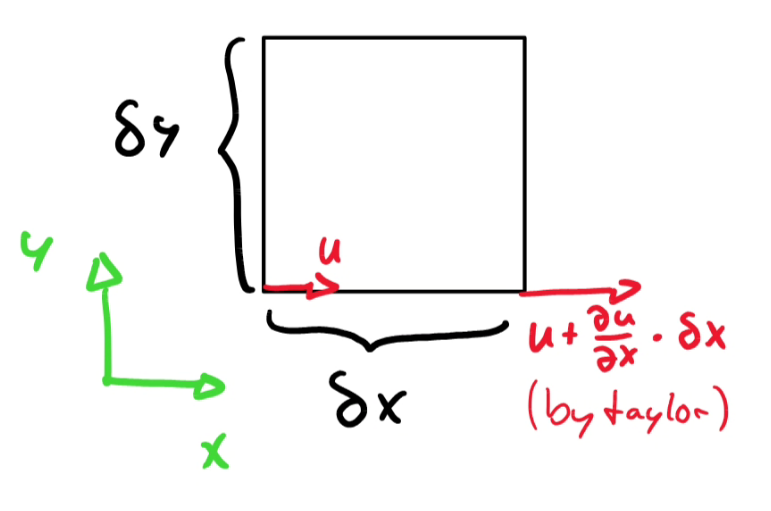
\includegraphics[width=0.4\linewidth]{Sketches/LinearDeformation}
		\caption{}
		\label{fig:lineardeformation}
	\end{figure}
	\begin{equation*}
		\frac{d(\delta x)}{d t} = \frac{\partial u}{\partial x} \implies \frac{1}{\delta x} \frac{d (\delta x)}{d t} = \frac{\partial u}{\partial x}
	\end{equation*}
	Likewise, $\partial_y v, \partial_z w$ are the linear deformations in $y$ and $z$, respectively. The volume change $\delta V = \delta x\cdot \delta y \cdot \delta z $ can be expressed as:
	\begin{equation*}
	\begin{split}
		   \frac{1}{\delta V}\frac{d(\delta V)}{dt}  
		&= \frac{1}{\delta x}\frac{d(\delta x)}{dt} + \frac{1}{\delta y}\frac{d(\delta y)}{dt}+\frac{1}{\delta z}\frac{d(\delta z)}{dt} \\
		&= \frac{\partial u}{\partial x} + \frac{\partial v}{\partial y } + \frac{\partial w}{\partial z}\\
		&= \nabla \cdot \vec v = 0\text{, if $\rho=const$}
	\end{split}
	\end{equation*}
	\item \textbf{angular deformations} (off-diagonal components of the gradient velocity tensor)
	\begin{figure}[H]
		\centering
		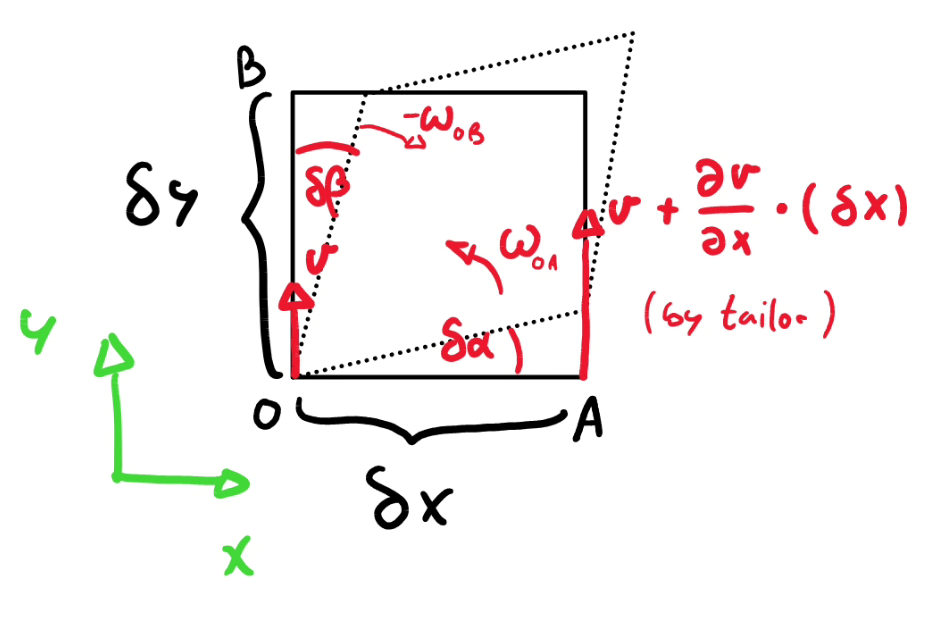
\includegraphics[width=0.4\linewidth]{Sketches/angular_deformations}
		\caption{}
		\label{fig:angulardeformations}
	\end{figure}
	\begin{equation*}
		\begin{split}
			\omega_{OA} &= \lim_{\Delta t \to 0}  \frac{\delta \alpha}{\Delta t} \stackrel{(*)}= \lim_{\Delta t \to 0} \frac{1}{\Delta t} \left(\frac{\frac{\partial v}{\partial x}\delta x \Delta t}{\delta x}\right) = \frac{\partial v}{\partial x}\\
			\omega_{OB} &= -\frac{\partial u}{\partial y}
		\end{split}
	\end{equation*}
	At $(*)$ we used a small angle approximation $\tan\delta \alpha \approx \delta \alpha$. The average rotation is the rotation of the bisecting line $\overline {OC}$. We can write it's angular velocity as
	\begin{equation*}
		\omega_z = \frac 12 \left(\omega_{OA}+\omega_{OB}\right) = \frac 12 \left(\frac{\partial v}{\partial x} - \frac{\partial u}{\partial y}\right)
	\end{equation*}
	Applying the same around $x$ and $y$ axis yields
	\begin{equation*}
		\vec \omega = \frac 12 \nabla \times \vec v = \frac 12 \zeta
	\end{equation*}
	in terms of the is the \textbf{vorticity} $\zeta$:\footnote{Heads up: Vorticity is not necessarily a circular transportation, but rather if (and how much) the fluid elements rotate about \textbf{their own axis}.}
	\begin{equation*}
		\boxed{\zeta = \nabla \times \vec v}
	\end{equation*}
	\textbf{Circularity} is a measure of velocity on some curve $c$ around an area $A$ on the surface of a volume.
	\begin{equation*}
		\Gamma = \oint_{c} \vec v \cdot \vec{ds} = \oint_{A} (\nabla \times \vec v )\cdot \vec{dA}
	\end{equation*}
	Where we see the vorticity again.
	It can be shown that inviscid flow means no change in rotation ($d\Gamma/dt=0$) and we say that "$\Gamma$ is conserved".
	
	It is therefore reasonable to consider inviscid flows ($\mu \to 0$) and irrotational flows ($\nabla \times \vec v = \vec 0$).
\end{itemize}


\section{Potential flow / Irrotational flow}
We assume that we are looking at \textit{incompressible, inviscid, and irrotational} flow.
We know that
\begin{equation*}
	\nabla \times \vec v = \vec 0\implies \exists \phi : \vec v = \nabla \phi
\end{equation*}
with the velocity potential $\phi$.

The continuity, and momentum equations turn into:
\begin{equation*}
	\begin{split}
		\text{Continuity Equation}\qquad\qquad\qquad\qquad\quad \nabla \cdot \vec v &= 0 \qquad (\rho = const) \\
		&\implies \boxed{\nabla^2 \phi = 0}\\\\
		\text{Momentum balance}\qquad\,\,\qquad \rho \left(\frac{\partial \vec v}{\partial t}+ \vec v \cdot \nabla \vec v \right) &= \rho \vec g - \nabla p \qquad \\
		\implies  \rho \frac{\partial \phi}{\partial t} + \frac{\rho}{2}v^2 + p + \rho g z &= const \qquad \Big | \text{steady:} \partial_t \phi = 0\\		
		\frac{\rho}{2}v^2 + p + \rho g z &= const
	\end{split}
\end{equation*}
Note that the result from the momentum balance is the same as the Bernoulli equation, but not restricted to any field lines.

To solve such a problem we follow the following steps:
\begin{enumerate}
	\setlength{\itemsep}{-5pt}
	\item \textbf{Solve Laplace} $\nabla^2\phi = 0$ with appropriate boundary conditions
	\item \textbf{Compute Velocity} $\vec v = \nabla \phi\implies \phi, \vec v$ known
	\item \textbf{Solve for the Pressure} Solve the momentum balance $\frac{\rho}{2}v^2 + p + \rho g z = const$ for pressure.
	\item \textbf{Integrate Pressure over Surface} to get the force on the object
\end{enumerate}


\section{2D Flows -- The Stream Function}
We start from the conservation of mass in an incompressible situation:
\begin{equation*}
	\begin{split}
		\nabla \cdot \vec v &= 0, \vec v = u\hat i + v\hat j + \cancel{w\hat k}\\
		\nabla \cdot \vec v &= 0 \Leftrightarrow \frac{\partial u}{\partial x} = - \frac{\partial v }{\partial y}\\
		\exists \Psi(x,y) :  \frac{\partial \Psi}{\partial y} &= u, -\frac{\partial \Psi}{\partial x} = v\implies \nabla \vec v = \frac{\partial}{\partial x}\frac{\partial \Psi}{\partial y} - \frac{\partial}{\partial y} \frac{\partial \Psi}{\partial x} = 0
	\end{split}
\end{equation*}
If we have a 2D-velocity field which is derived from a so-called \textbf{Stream Function} $\Psi$, it automatically satisfies mass conservation.

To observe places, where the $\Psi$ is constant, the exact differential of $\Psi$ can be expressed as:
\begin{equation*}
	d\Psi = \frac{\partial \Psi}{\partial x}\cdot dx + \frac{\partial \Psi}{\partial y}\cdot dy = 0\Leftrightarrow \frac{dy}{dx} = \frac{v}{u}\quad \text{eq. of a streamline}
\end{equation*}
Therefore, a stream function is constant along a stream line.

\section{2D Potential Flow}
If we assume the following things
\begin{itemize}
	\setlength{\itemsep}{-5pt}
	\item incompressible
	\item inviscid
	\item irrotational $\implies \vec v = \nabla \phi$
	\item 2d $\implies $ there is a stream function $\Psi$
\end{itemize}
We can therefore combine
\begin{equation*}
	\begin{split}
		\phi:\qquad 0 &= \nabla \cdot \vec v = \nabla^2 \phi \\
		\implies 0&=\frac{\partial^2 \phi}{\partial x^2}+ \frac{\partial ^2 \phi}{\partial y^2} \\
		\Psi: \qquad \vec 0 &= \nabla \times \vec v\\\implies 0 &= \frac{\partial ^2 \psi}{\partial x^2}+ \frac{\partial ^2 \psi}{\partial y^2}
	\end{split}
\end{equation*}
Both the stream function and the velocity potential satisfy the Laplace equation\footnote{They don't need to be the same yet, as the boundary conditions are not clear.}

To compare them, we compare their differential:
\begin{equation*}
	d\phi  = u dx + v dy = 0\implies \frac{d y}{dx} = -\frac{u}v
\end{equation*}
the slope is the negative inverse of the stream function, meaning they are orthogonal to the stream lines. From this follows that:

\shadowbox{Equipotential lines ($\phi = const$) are perpendicular to stream lines ($\psi = const$).}

\begin{figure}[H]
	\centering
	\begin{subfigure}{0.48\linewidth}
		\centering
		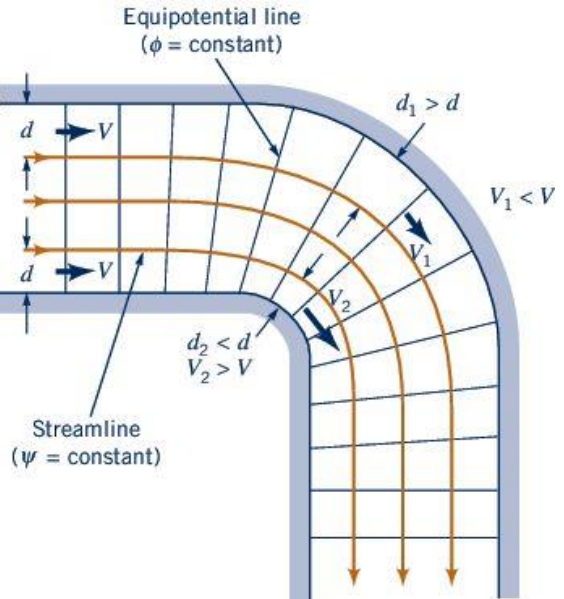
\includegraphics[height=5cm]{Sketches/equipotential_lines_1}
		\caption{streamline and equipotential line illustrated around a curve}
		\label{fig:equipotentiallines1}
	\end{subfigure}%
	\hfill
	\begin{subfigure}{0.48\linewidth}
		\centering
		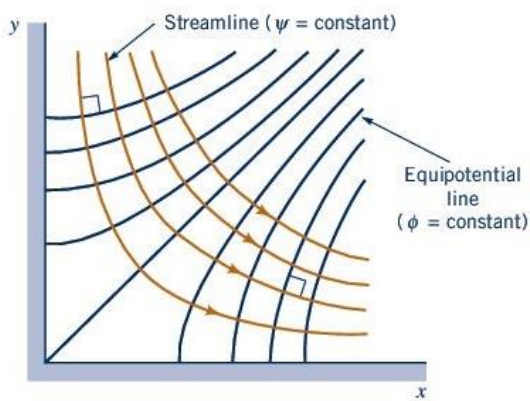
\includegraphics[height=5cm]{Sketches/equipotential_lines_2}
		\caption{streamline and equipotential line illustrated in a corner}
		\label{fig:equipotentiallines2}
	\end{subfigure}
\end{figure}

\paragraph{Example}
Given $\phi = \frac a2 (x^2-y^2)$, we calculate $\partial^2_{xx}\phi + \partial^2_{yy}\phi = a-a = 0$ to verify that it satisfies the condition for a velocity potential. We can den try to determine the stream function $\psi$, by their relationship via $u$ and $v$:
\begin{equation*}
	\left.\begin{split}
		u &= \frac{\partial \phi}{\partial x} = ax = \frac{\partial \psi}{\partial y}\\
		v &= \frac{\partial \phi}{\partial y} = -ay = -\frac{\partial \psi}{\partial x}
	\end{split}\right\} \Psi = axy + \cancel c
\end{equation*}
The constant has no physical meaning, and can be chosen arbitrarily (zero is the simplest one choice.)




\subsection{Basic plane potential flows}
If we can construct a potential-flow solution, such that the stream line captures a desired surface of a 2D body, then boundary conditions are satisfied on the surface. These flow solutions can be superimposed to get more complex solutions.

We will discuss four flows
\subsubsection{Uniform Flow}
\begin{equation*}
	\begin{split}
		\phi &= U_0\cdot x\\
		\psi &= U_0\cdot y
	\end{split}
\end{equation*}
\begin{figure}[H]
	\centering
	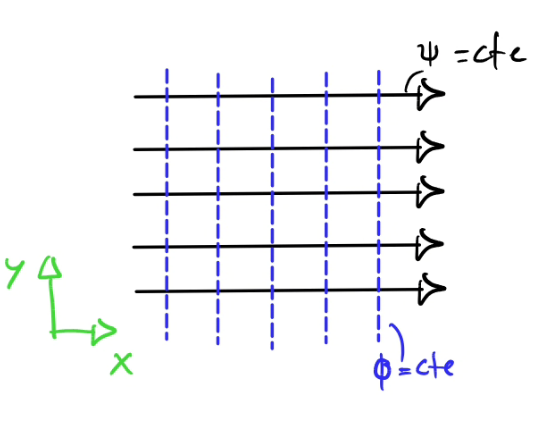
\includegraphics[width=0.4\linewidth]{Sketches/uniform_flow}
	\caption{}
	\label{fig:uniformflow}
\end{figure}

\subsubsection{Line-Source and -Sink}
At a point in space (here the origin), a volume rate $m$ is emerging. 
\begin{equation*}
	\left.\begin{split}
		v_r&= \frac{m}{2\pi r} =  \frac{\partial \phi}{\partial r} = \frac 1r \frac{\partial \Psi}{\partial \theta}\\
		v_\theta &= 0 = \frac 1r \frac{\partial \phi}{\partial \theta} = -\frac{\partial \Psi}{\partial r}
	\end{split}\right\}\implies \begin{cases}
	\phi =\frac{m}{2\pi}\ln r \\
	\psi = \frac{m}{2\pi}\theta
	\end{cases}\hfill
\end{equation*}
\begin{figure}[H]
	\centering
	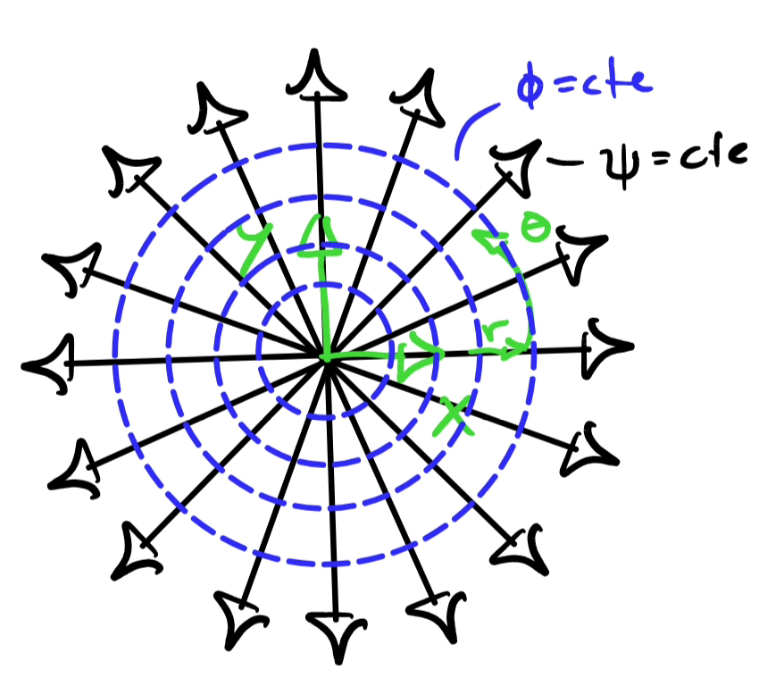
\includegraphics[width=0.4\linewidth]{Sketches/source_sink_flow}
	\caption{}
	\label{fig:sourcesinkflow}
\end{figure}


\subsubsection{Line Vortex}
\begin{equation*}
	\left.\begin{split}
		v_\theta&= \frac{m}{2\pi r} =  \frac 1r \frac{\partial \phi}{\partial \theta} = -\frac{\partial \Psi}{\partial r}\\
		v_r &= 0 = \frac{\partial \phi}{\partial r} = \frac 1r \frac{\partial \Psi}{\partial \theta}
	\end{split}\right\}\implies \begin{cases}
		\phi =k\theta \\
		\psi = -k\ln r
	\end{cases}\hfill
\end{equation*}
\begin{figure}[H]
	\centering
	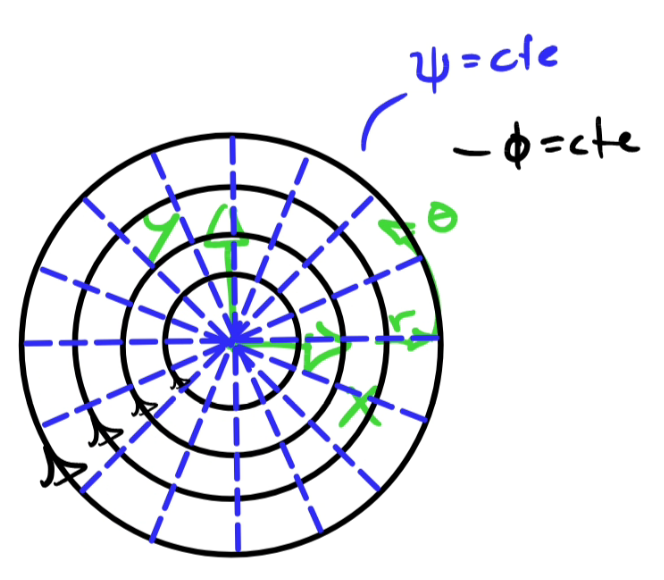
\includegraphics[width=0.4\linewidth]{Sketches/line_vortex_flow}
	\caption{}
	\label{fig:linevortexflow}
\end{figure}

\subsubsection{Doublet}
This is actually already a superposition. Combining a source and a sink at equal distance from the origin of opposite but equal strength. To neglect angular problems, we look at the case where the distance $a$ goes to zero, and the volume rate $m$ to infinity, such that $m\cdot a = const$.
\begin{equation*}
	\begin{split}
		\phi = -\frac{m}{2\pi}(\theta_1-\theta_2) &\stackrel{a\to 0}{\longrightarrow}\frac{k\cos\theta}r\\
	\psi &\stackrel{a\to 0}{\longrightarrow} -\frac{k\sin\theta}{r}
	\end{split}\qquad k = \frac{ma}{\pi}
\end{equation*}

\begin{figure}[H]
	\centering
	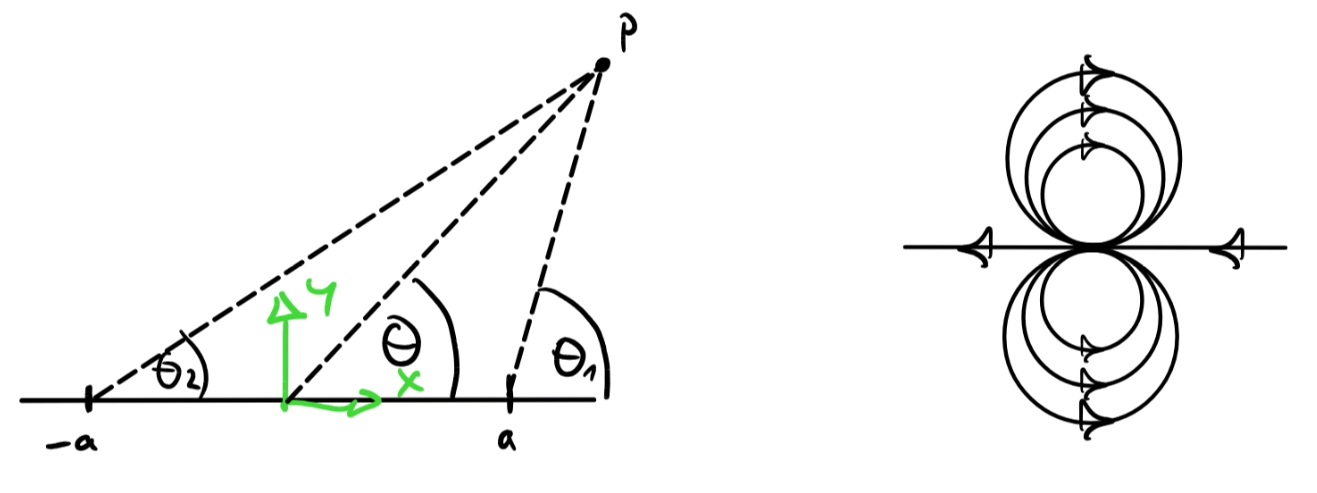
\includegraphics[width=0.4\linewidth]{Sketches/doublet_flow}
	\caption{}
	\label{fig:doubletflow}
\end{figure}
\begin{tabular}{|m{2cm}|l|l|m{4cm}|}
	\hline
	\textbf{Description of Flow Field} & \textbf{Velocity Potential} & \textbf{Stream Function} & \textbf{Velocity Components} \\
	\hline
	Uniform flow at angle $\alpha$ with the $x$ axis &
	$\phi = U(x \cos \alpha + y \sin \alpha)$ &
	$\psi = U(y \cos \alpha - x \sin \alpha)$ &
	$u = U \cos \alpha$ \newline $v = U \sin \alpha$ \\
	\hline
	Source or sink \newline $m > 0$ source \newline $m < 0$ sink &
	$\phi = \dfrac{m}{2\pi} \ln r$ &
	$\psi = \dfrac{m}{2\pi} \theta$ &
	$v_r = \dfrac{m}{2\pi r}$ \newline $v_\theta = 0$ \\
	\hline
	Free vortex \newline $\Gamma > 0$ counterclockwise \newline $\Gamma < 0$ clockwise &
	$\phi = \dfrac{\Gamma}{2\pi} \theta$ &
	$\psi = -\dfrac{\Gamma}{2\pi} \ln r$ &
	$v_r = 0$ \newline $v_\theta = \dfrac{\Gamma}{2\pi r}$ \\
	\hline
	Doublet &
	$\phi = \dfrac{K \cos \theta}{r}$ &
	$\psi = -\dfrac{K \sin \theta}{r}$ &
	$v_r = -\dfrac{K \cos \theta}{r^2}$ \newline $v_\theta = -\dfrac{K \sin \theta}{r^2}$ \\
	\hline
\end{tabular}
\subsection{Superpositions}
\subsubsection{The Half-Body}
This is a superposition of a source and a uniform flow.
Through linearity, the stream function for this combination is:
\begin{equation*}
	\begin{split}
		\psi &= \psi_{UF} + \psi_{S}\\
		&= U_0\cdot y + \frac{m}{2\pi}\theta \\
		&= U_0r\sin\theta + \frac{m}{2\pi}\theta
	\end{split}
\end{equation*}
The velocity potential $\phi$ can be described similarly through
\begin{equation*}
	\begin{split}
		\phi &= \phi_{UF} + \phi_{S}\\
		&=U_0r\sin\theta + \frac{m}{2\pi}\ln r 
	\end{split}
\end{equation*}

Through these definitions of $\phi$ and $\psi$, we can express the velocities as follows:
\begin{equation*}
	\begin{split}
		v_r &= \frac 1r \frac{\partial \psi}{\partial \theta } = U_0 \cos\theta + \frac{m}{2\pi r}\\
		v_\theta &= - \frac{\partial \psi}{\partial r} = -U_0\sin\theta 
	\end{split}
\end{equation*}

To understand these velocities, we find the stagnation point on the x-axis, at $\theta_{sp}=\pi$, $v_r= 0$:
\begin{equation*}
	0=u_0\cos\theta_{sp} + \frac{m}{2\pi r_{sp}} \implies r_{sp} = \frac{m}{2\pi U_0}
\end{equation*}
\begin{figure}[H]
	\centering
	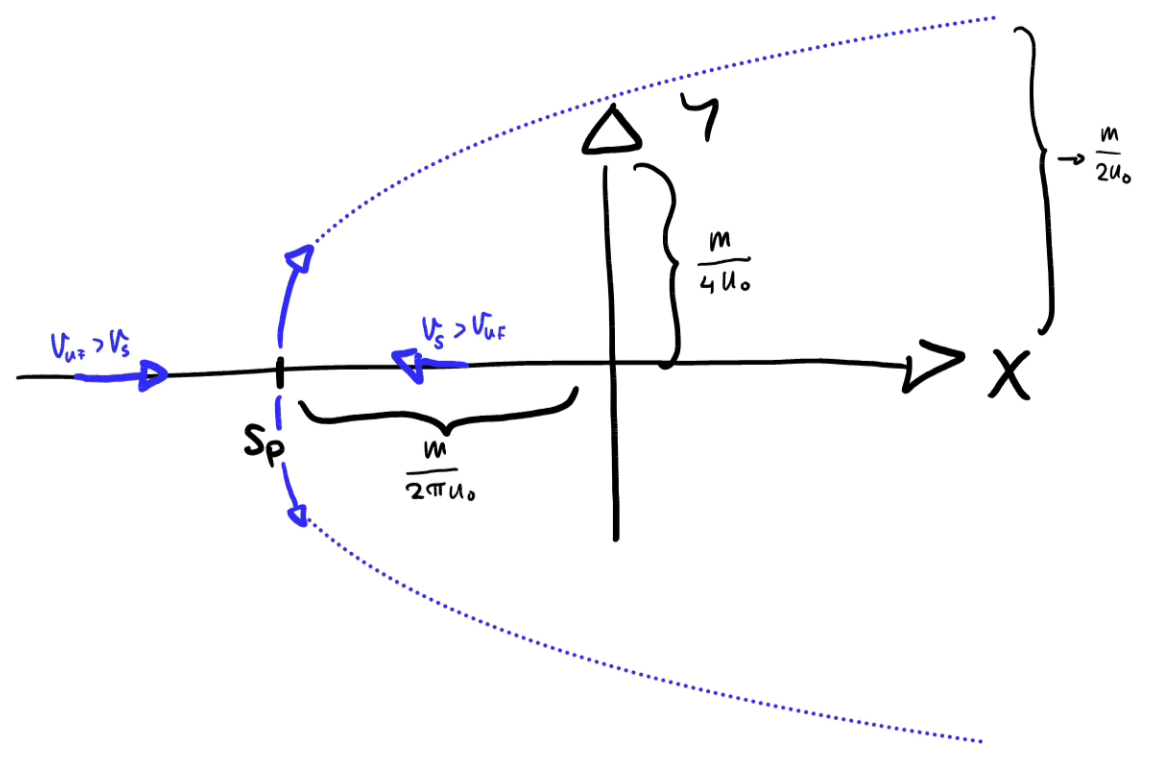
\includegraphics[width=0.4\linewidth]{Sketches/halfbody}
	\caption{}
	\label{fig:halfbody}
\end{figure}
Describing the stagnation stream line, we write
\begin{equation*}
	\psi_{sp} = \frac m2 = U_0 r \sin\theta + \frac{m}{2\pi}\theta \implies r = \frac{m}{2\pi U_0} \frac{\pi - \theta}{\sin\theta},\quad \theta \in[0,2\pi[
\end{equation*}

The intersection point of the stagnation stream line on the $y$ axis is at $\theta=\pi/2$, with radius $r=\frac{m}{4U_0}$.
To inspect the y-height of the stagnation stream line, we get $y=r\sin\theta = \frac{m}{2\pi U_0}(\pi-\theta) = \frac{m}{2 U_0}$.

We interpret the stagnation stream line as the surface of a so-called \textit{half-body}.

Next we would like to calculate the velocity and pressure on the surface
\begin{equation*}
	v^2 + v_r^2 + v_\theta ^2 = U_0^2 \left(1+2\frac{b}{r}\cos(\theta) + \frac{b^2}{r^2}\right), \qquad b = \frac{m}{2\pi U_0}
\end{equation*}

\subsubsection{Rankine Oval}
A source and sink placed at $x=-a$ and $x=a$ respectively, all inside of a uniform flow. This will not be discussed, further reference can be found in \textbf{Munson 6.6.2}.

\subsubsection{Circular Cylinder}
We superimpose uniform flow and a doublet. We can immediately write the stream function and velocity potential
\begin{equation*}
	\begin{split}
		\psi &= \psi_{UF} + \psi_{D} = U_0y - \frac{K\sin\theta}{r} = \left(U_0+\frac{K}{r^2}\right)r\sin\theta\\
		\phi &= \phi_{UF} + \phi_D = \left(U_0+\frac K{r^2}\right)r\cos\theta
	\end{split}
\end{equation*}

We have two stagnation points for $y=0$, $\theta\in\{0,\pi\}$. $\psi=0$ is a stream line through $r=a$ if $u_0-\frac K{r^2}=0$. We need to choose $K=U_0a^2$, such that the stagnation stream line is a circle with radius $a$. The flow around a cylinder of radius $a$ can be described as:
\begin{equation*}
	\begin{split}
		\psi = U_0 \left(1-\frac{a^2}{r^2}\right) r \sin\theta\\
		\phi = U_0 \left(1+\frac{a^2}{r^2}\right)r \cos\theta
	\end{split}
\end{equation*}

The velocity can be written as
\begin{equation*}
	\begin{split}
		 v_r &= \frac{\partial \phi}{\partial r} = \frac{1}{r}\frac{\partial \psi}{\partial \theta }=U_0\left(1-\frac{a^2}{r^2}\right)\cos\theta\\
		 v_\theta &= \frac{1}{r}\frac{\partial \phi}{\partial \theta} = -\frac{\partial \psi}{\partial r} = - U_0\left(1+\frac{a^2}{r^2}\right) r \sin\theta
	\end{split}
\end{equation*}
On the surface of the cylinder ($a=r$), we get $v_r = 0$ and $v_\theta = 2a \sin\theta$. This is okay, as the flow is assumed to be inviscid. 

To calculate the pressure $p_s$ on the surface, we use newton's second law:
\begin{equation*}
	\begin{split}
		\rho \frac{\partial \phi}{\partial t}+ \frac{\rho}{2}|\vec v|^2 + p + \cancel{\rho gz}^{\text{negl.}} &= const\\
		p_0 + \frac 1 2\rho U_0^2 &= p_s + \frac 12 \rho v_{\theta}^2\\
		\implies p_s&=p_0 + \frac 12 \rho U_0^2\left(1-4\sin^2\theta\right)
	\end{split}
\end{equation*}
\paragraph{Drag and Lift Forces}
\begin{equation*}
	\begin{split}
		F_L &= F_y = -\int_0^{2\pi}p_s\sin\theta a\,d\theta = 0\implies\text{no lift}\\
		F_D & =F_x =  \int_0^{2\pi}p_s\cos\theta a \,d\theta = 0 \implies \text{no drag}
	\end{split}
\end{equation*}
The result of no drag is called d'Alembert's Paradox and is only true because we assume inviscid flow. For real-world scenarios, the effects of viscosity result in a non-zero drag force. 

\subsubsection{Rotating Cylinder}
In order to create lift, the up-down symmetry needs to be broken. Adding a vortex helps doing this.
\begin{equation*}
	\begin{split}
		\psi &= U_0\left(1-\frac{a^2}{r^2}\right)r\sin\theta - \frac \Gamma {2\pi}\ln r\\
		\phi &= U_0\left(1+\frac{a^2}{r^2}\right)r\sin\theta - \frac \Gamma {2\pi} r\\
	\end{split}
\end{equation*}
On the surface ($r=a$), the velocity becomes:
\begin{equation*}
	\begin{split}
		v_{r,s} = \frac{1}{r}\frac{\partial \psi}{\partial \theta}\Big|_{r=a} = 0\\
		v_{\theta,s} &= -\frac{\partial \psi}{\partial r} \Big|_{r=a} = -2U_0 \sin\theta + \frac{\Gamma}{2\pi a}
	\end{split}
\end{equation*}
At the stagnation point on the cylinder surface, 
\begin{equation*}
	\sin\theta_{sp} = \frac{\Gamma}{2\pi U_0 a}
\end{equation*}
This describes the following points:
\begin{figure}[H]
	\centering
	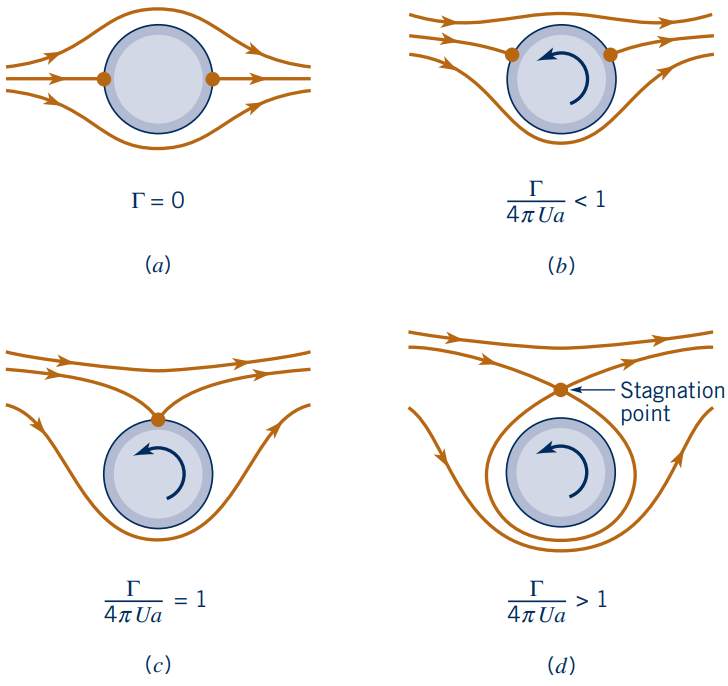
\includegraphics[width=0.4\linewidth]{Sketches/rotating_cylinder_stagnation_points}
	\caption{Munson et.al.}
	\label{fig:rotatingcylinderstagnationpoints}
\end{figure}
The pressure on the surface is
\begin{equation*}
	p_s = p_1 + \frac 12 \rho U_0^2 \left(1-4\sin^2\theta + \frac{2\Gamma\sin\theta}{2\pi a U_0}-\frac{\Gamma^2}{4\pi^2 a^2 U_0^2}\right)
\end{equation*}
This still has symmetries around $\pi/2, 3\pi/2$, and therefore doesn't generate drag. However, the symmetry from $y$ to $-y$ is broken.
This leads to the following lift force:
\begin{equation*}
	F_L = -\int_0^{2\pi} p_s \sin\theta a\,d\theta= -\frac{1}{2}\rho U_0^2\int_0^{2\pi} \frac{2\Gamma \sin\theta}{2\pi a U_0} - \frac{\Gamma^2}{4\pi^2 a^2 U_0^2}a\sin\theta \,d\theta = -\rho U_0 \Gamma
\end{equation*}
Which is the \textbf{Magnus Effect}:
\begin{equation*}
	\boxed{F_L = -\rho U_0 \Gamma}
\end{equation*}
The lift force (perpendicular to the flow direction) per "span" is given by $-\rho U_0 \Gamma$.
When the flow comes from the left, $\Gamma$ must be negative (clockwise) in order for the lift to be positive.
\subsection{Lift and drag on an Airfoil}
\footnotesize{Munson chapter 9}

An airplane flies at high Reynolds numbers, viscosity can be ignored. For inviscid potential flow and infinite wings (that can therefore be observed in 2D), then the general results:
\begin{equation*}
	\begin{aligned}
		F_L &= -\rho U_0 \Gamma &&\textbf{lift per unit span}\\
		F_D &= 0 && \textbf{d'Alembert's paradox}
	\end{aligned}
\end{equation*}

For any closed curve around the airfoil:
\begin{equation*}
	\Gamma = \oint_c \vec v \cdot \vec{ds}
\end{equation*}
are valid for any shape of airfoil.\footnote{By the Kutta-Joukowski theorem} The Kutta-condition chooses the stagnation point to be pinned at the sharp feature on the trailing edge. This limits the infinite solutions resulting from inviscid flow to the solution chosen in nature, where viscosity is still important at high velocities very close to surfaces. Stalling is when the Kutta-condition can no longer be satisfied and no lift is generated.

\section{Viscous Flow}
Recall the equations for incompressible Newtonian fluids:
\begin{equation*}
\begin{split}
		\rho \frac{\partial \vec v}{\partial t}+ \rho \vec v \cdot \nabla \vec v &= -\nabla p + \rho \vec g + \underbrace{\mu \nabla^2 \vec v }_{\text{Viscous term}}\\
		\nabla \cdot \vec v &= 0
\end{split}
\end{equation*}
Viscosity by itself implies the no-slip condition boundary condition at the walls: 
\begin{equation*}
	\vec v = \vec v_{wall}
\end{equation*}

The above equation is very hard to solve, they are non-linear and thus in general impossible to solve. In few specific cases, we can however find solutions to them.
\subsection{Laminar shear flow between parallel plates}
Consider two parallel plates at distance $h$, where one of them moves at velocity $v_0$. The downstream direction is $\hat x$. 

The assumptions of laminar flow are made, which assumes that the solution is of the form $\vec v (\vec r,t)= u(y,t)\hat i$. It only has a downstream component and only depends on $y$, which is the wall-normal coordinate. 

Under these assumptions, the non-linear term vanishes
\begin{equation*}
	\vec v \cdot \nabla \vec v = u(y,t)\frac{\partial}{\partial x}u(y,t)\hat i = \vec 0
\end{equation*}

Furthermore, we assume that there is a constant prescribed pressure gradient along $x$:
\begin{equation*}
	\frac{\partial p}{\partial x} = cte\qquad \frac{\partial p}{\partial z} = 0
\end{equation*}
plugging this into the continuity equation yields
\begin{equation*}
	\nabla \cdot \vec v = \frac{\partial u}{\partial x} + \frac{\partial v}{\partial y} + \frac{\partial w}{\partial z} = 0
\end{equation*}
The moment conservation equation results in
\begin{equation*}
	\begin{split}
		\rho \frac{\partial u}{\partial t}\hat i + \vec 0 &= - \frac{\partial p}{\partial x}\hat i - \frac{\partial p}{\partial y}\hat j - \rho g\hat j + \mu \left(\frac{\partial^2 }{\partial x^2 }+\frac{\partial^2 }{\partial y^2 }+\frac{\partial^2 }{\partial z^2 }\right)u \hat i\\
		\hat i: \qquad \rho \frac{\partial u}{\partial t}&=-\frac{\partial p}{\partial x}+ \mu \frac{\partial^2 }{\partial y^2}u\\
		\hat j:\qquad 0 &= -\frac{\partial p}{\partial y}-\rho g\\
		\hat k: \qquad 0 &= 0\\\\
		\implies p &= -\rho g y + \frac{\partial p}{\partial x}x + C\\
		&= -\rho g y + c
	\end{split}
\end{equation*}
What is left to solve is
\begin{equation*}
	\rho \frac{\partial u}{\partial t} = \mu \frac{\partial ^2}{\partial y^2}u - \frac{\partial p}{\partial x}
\end{equation*}
We can recognise this as a diffusion equation for momentum density with diffusion coefficient $\mu/\rho = \nu$.

\paragraph{Steady State Solutions}
There are three possible combinations:
\begin{itemize}
	\setlength{\itemsep}{-5pt}
	\item \textbf{plane Poiseuille flow} $u_0=0,\partial_xp \ne 0$\\
	\item \textbf{plane Couette flow} $u_0\ne0 ,\partial_xp =0$\\
	\item \textbf{mixed Couette flow} $u_0\ne0,\partial_xp \ne 0$
\end{itemize}

For each of these, we need to solve
\begin{equation*}
	\begin{cases}
		0=\mu \frac{d^2u}{dy^2}- \frac{\partial p}{\partial x}\\
		u(y=-h) = 0\\
		u(y=h) = u_0
	\end{cases}
\end{equation*}
Which results in 
\begin{equation*}
	\begin{split}
		u &= \frac{1}{2\mu}\left(\frac{\partial p}{\partial x}\right) y^2 + C_1 y + C_2\\\implies
		u(y)&=\frac{u_0}{2}\left(\frac{y}{h} + 1\right)+ \frac{1}{2\mu }\left(\frac{\partial p}{\partial x}\right)\left(y^2 -h^2\right)
	\end{split}
\end{equation*}

The volumetric flow rate (per unit depth) is 
\begin{equation*}
	Q= \int_{-h}^h u\,dy = u_0 h- \frac{2}{\mu} \left(\frac{\partial p}{\partial x}\right)\frac{h^3}{3}
\end{equation*}
\paragraph{Time Dependant Solution}
This can be solved exactly like the diffusion equation. 
\subsection{Pipe Flow}
Assume we have a cylindrical pipe or radius $R$. We impose a cylindrical coordinate system to write the assumptions:
\begin{itemize}
	\setlength{\itemsep}{-5pt}
	\item incompressible,  Newtonian
	\item laminar
	\item steady
	\item $\partial_z p = cte$ (incompressible)
\end{itemize}

From laminar and steady, we conclude
\begin{equation*}
	\begin{split}
		\vec v = V_z (r)\hat z\\
		\nabla \cdot \vec v = 0
	\end{split}
\end{equation*}
the Navier-Stokes equations turn into
\begin{equation*}
	0 = -\partial_zp + \mu \left(\frac 1r \frac{\partial }{\partial r}\left(r \frac{\partial V_z}{\partial r}\right)\right)\\
	\implies V_z = \frac{1}{4\mu}\left(\frac{\partial p}{\partial z}\right) r^2+ c_1\ln r + c_2
\end{equation*}
Through the boundary conditions
\begin{equation*}
	\begin{cases}
		V_z|_{r=R} = 0&(1)\\
		|v_z|_{r=0}< \infty &(2)
	\end{cases}
\end{equation*}
we conclude that by $(1)$ $c_1 = 0$ and by $(2)$:
\begin{equation*}
	c_2 = -\frac{1}{4\mu}\left(\frac{\partial p}{\partial z}\right)R^2
\end{equation*}
and therefore
\begin{equation*}
\boxed{	V_z = \frac{1}{4\mu}\left(\frac{\partial p}{\partial z}\right)(r^2-R^2)}
\end{equation*}

\end{document}
